% master.tex : master-fil for projektet
% ------------------------------------------------------------------------------
% Dette er hovedfilen for projektet, hvori indhold fra alle input-filer (tekst,
% billeder, litteraturdatabaser, osv.) samles

% Dokumenttypen 'book' er valgt pga. dens mange fleksible indstillinger
% Se https://tex.stackexchange.com/a/36989/118167
\documentclass[11pt,a4paper,twoside,openright,danish]{book}

% Variabler, som bruges til automatisk at indsætte titel, forfattere, osv. på
% forsiden og titelbladet.
\def \projecttitle       {Traveling Salesperson Problem}
\def \projectsubtitle    {Grafteori}
\def \projecttheme       {Grafteori}
\def \projectdegree      {Matematik}  % eller Matematik-Økonomi/Teknologi
\def \projectperiod      {Efterårssemesteret 2019}
\def \projectnumber      {P1}
\def \projectgroup       {C2-20}
\def \projectauthors     {
	Anne Bang Christensen\\
  Caroline Nørskov Budsted Weje\\
  Daniel Bursac Hasanovic\\
  Ebbe Michelsen\\
  Henriette Høiberg Bjørn\\
	Mie Frederiksen Larsen\\
	Sigrid Schrøder Jensen
}
\def \projectsupervisors {
	Anne Marie Svane
  % ...
}

% Preamblet indeholder alle de indstillinger og makroer, som skal indsættes for
% hovedindholdet, og i denne skabelon samles det i filen aaumath.sty, som
% definerer en pakke, der kan indlæses med \usepackage.
\usepackage{aaumath}

\usetikzlibrary{automata,positioning}

% Dokumentets indhold indsættes mellem \begin- og \end-makroerne for
% 'document'-blokken
\begin{document}

% Dokumentets 'front matter' tælles ikke med ifm. antal sider og nummereres med
% romerske tal. Herunder hører f.eks. forsiden, titelbladet, forordet og
% indholdsfortegnelsen.
\frontmatter
% incl/misc/frontpage.tex : rapportens forside
% ------------------------------------------------------------------------------


\backgroundsetup{
  scale = 1,
  angle=0,
  opacity=1,
  contents = {
    
\includegraphics[width=\paperwidth,height=\paperheight]{fig/img/aau/waves.pdf}
  }
}
\BgThispage
\pdfbookmark[0]{Forside}{forside}
\begin{titlepage}
  \centering
  \phantom{}
  \vspace{2cm}

  % AAU-segl
  \begin{minipage}[c]{0.2\paperwidth}
    \centering
    \makebox[0pt]{
      % fig/tikz/aau-badge.tex : AAU-logo til forsiden
% ------------------------------------------------------------------------------

\begin{tikzpicture}
  % Tegn hvid cirkel og tilføj det gennemsigtige, blå logo ovenpå
  \node[circle,color=white,fill=white,minimum size=1.175\textwidth] at (0,0) {};
  \node at (0,0) {
\includegraphics[width=\textwidth]{fig/img/aau/logo-circle.pdf}};
\end{tikzpicture}

    }
  \end{minipage}

  % Hovedindhold
  \vspace{4cm}
  {\fontfamily{bch}\selectfont
    \fboxsep0pt\colorbox{white}{
      \begin{minipage}{\textwidth}
        \centering
        \color{AAUblue1}

        \vspace{2em}
        {\Huge\bfseries\projecttitle}

        {\Large\bfseries\projectsubtitle}

        \bigskip
        \parbox{\textwidth}{\centering\large\projectauthors}

        \bigskip
        {\bfseries\large{\projectnumber}-Projekt, Gruppe \projectgroup, \projectdegree}
        \vspace{2em}
      \end{minipage}
    }
  }

\end{titlepage}

% incl/misc/titlepage.tex : rapportens titelblad
% ------------------------------------------------------------------------------
% Titelbladet genereres af makroen \aautitlepage, som er defineret i
% /incl/pre/ext/aautitlepage.sty


\pdfbookmark[0]{Titelblad}{titelblad}
\aautitlepage{
  \projectinfo{
    \projecttitle
  }{
    \projecttheme
  }{
    \projectperiod
  }{
    Gruppe \projectgroup
  }{
    \parbox[t]{\textwidth}{\projectauthors}
  }{
    \parbox[t]{\textwidth}{\projectsupervisors}
  }{
    \today
  }
}{
  \textbf{Institut for Matematiske Fag}\\
  Skjernvej 4A\\
  DK-9220 Aalborg Ø\\
  \href{http://math.aau.dk}{http://math.aau.dk}
}{
  % incl/misc/abstract.tex : projektets abstract
% ------------------------------------------------------------------------------
% Et abstract er et kort resume af rapporten, som vises på titelbladet

In discrete mathematics, the famous problem Travelling Salesperson Problem (TSP) states the task of optimizing a route between different cities in terms of travelled distance. 
When applying concepts from graph theory, solving TSP is equivalent to finding the shortest possible simple circuit through all vertices in a complete weighted graph, which is called a Hamilton circuit. 
For solving many mathematical problems, algorithms can be implemented. Algorithms are precisely defined steps that together make up the calculations for finding a solution. 
Not all algorithms are equally efficient. For making it possible to compare different algorithms, Big-$O$, Big-$\Omega$ and Big-$\Theta$ notations are introduced together with the term time complexity. 
Algorithms with polynomial time complexity can solve a problem relatively fast. 
However, it is not possible to solve TSP with a polynomial algorithm, which means finding an optimal solution can be an unreasonably slow task for a larger number of cities. 
Instead, a solution to TSP can be estimated by approximation algorithms.
Even though they lack precision, these algorithms can give a solution to TSP in polynomial time. 

}

% incl/misc/contents.tex :
% ------------------------------------------------------------------------------

\pdfbookmark[0]{Indhold}{indhold}

% Indstillingerne i denne fil er grupperet, så de ikke påvirker andre dele
\begingroup

% Slå twoside fra midlertidigt for at undgår sideskift
\makeatletter
\@twosidefalse
\makeatother

% Placer indholdsfortegnelsen på sin egen side (bedst når den kun fylder en side)
\tableofcontents
\clearpage

% Placer oversigtslisterne på efterfølgende sider
\let\clearpage\relax
\listoffigures
\listoftables
\listofalgorithms
\lstlistoflistings

\endgroup


% Dokumentets 'main matter' (hovedindhold) er der, hvor det meste indhold skal
% sættes ind. Sider og overskrifter er nummererede med arabiske tal.
\mainmatter

% Input-filer bør opdeles således, at hver fil svarer til et kapitel. Makroen
% \include indsætter et sideskift og indholdet fra den givne stil.

% \include{incl/main/example1}
% \include{incl/main/example2}
% ...

\chapter{Indledning}
Et stort problem indenfor matematikken er Travelling Salesperson Problem. 
Dette er et problem, der handler om at finde den kortest mulige kreds i en graf. 
For at undersøge dette problem, skal der bruges toeri om blandt andet algoritmer, kompleksitet og grafer.
Algoritmer bruges til at løse matematiske problemer via en række af skridt der skal genneføres. 
Algoritmer skal bruges for at komme med forslag til en løsningsalgoritme til Travelling Salesperson Problem. 
For at finde ud af, hvor kompliceret en algoritme er, udregner man algoritmens kompleksitet. 
Dette bruges, til at undersøge hvor effektiv en løsningsalgoritme til Travelling Salesperson Problem er. 
Grafer bruges til at vise sammenhænge. 
I tilfældes med Travelling Salesperson Problem, bruges grafer til at vise, hvordan byer og steder ligger i forhold til hinanden og hvordan de er forbundet. 
I dette projekt vil der blive fokuseret meget på teorien der ligger bag Travellign Salesperson Problem.\\

\noindent \textbf{Problemformulering} \\
Hvordan kan teori om algoritmer, kompleksitet og grafer bruges til at løse Travelling Salesperson Problem?
\\\\
Hvad er algoritmer, kompleksitet, induktionsbeviser og grafer? Hvordan kan Travelling Salesperson Problem repræsenteres ved hjælp af grafteori, og hvorledes kan et løsningsforslag til Travelling Salesperson Problem approksimeres?
\\\\


\chapter{Algoritmer}
Dette kapitel tager udgangspunkt i \citep{dmat}, medmindre andet er angivet.

Mange matematiske problemer kan ikke løses ved hjælp af en simpel beregning, men kræver i stedet en række af skridt, der giver en løsning til problemet. 
En beskrivelse af den nødvendige sekvens af skridt kaldes en algoritme. 


\begin{defn}
En algoritme er et endeligt sæt af præcise instruktioner, som beskriver udførelsen af en beregning eller løsning af et problem.
\end{defn}

I denne rapport vil der blive brugt pseudokode til at beskrive, hvordan en algoritme kan opstilles i computersprog. 
En pseudokode kan let oversættes til et ønsket programmeringssprog og kan let læses og forstås. 
I dette kapitel vil tre algoritmer blive beskrevet for at give en ide om, hvad en algoritme kan bruges til. 

\section{Eksempler på algoritmer}
\subsection{Søgealgoritme}
Skal den største værdi i en liste findes, kan det gøres med en algoritme. 
Selvom det kan virke meget simpelt at læse en liste igennem og finde det største tal, kan det blive problematisk og tidskrævende, hvis der er tale om en længere liste. 
Derfor kan en algoritme være smart, da nogle algoritmer hurtigt kan gennemgå lange lister. 
Desuden kan en algoritme løses af en computer, hvilket også gør det nemmere. 

En sådan algoritme kan udføres ved at sætte det første element lig med en variabel $maks$. 
Dernæst sammenlignes denne værdi med det næste element, som  $maks$ overtager, hvis det er større end den nuværende værdi af $maks$. 
Er det næste element mindre end det nuværende $maks$, sker der ikke noget, og der fortsættes til det næste element i listen. 
Dette gentages indtil hele listen er gennemgået, hvorefter $maks$ returneres.

Herunder ses et eksempel på hvordan en sådan søgealgortime kan skrives med pseudokode:


\begin{algorithm}
\caption{Find maksimalt element i en liste}
\label{find_maks}
\textbf{procedure} $ maks(a_1, a_2, ..., a_n) $

$ maks:=a_1 $ \\
\textbf{for} $i :=2$ \textbf{til} $n$ \\
$\-$ $\-$ $\-$ $\-$ $\-$ $\-$
\textbf{hvis} $maks<a_i$ \textbf{så}
$maks:=a_i$ \\
\textbf{returnér} $maks \, \lbrace maks$ er det største element $\rbrace$
\end{algorithm}

\subsection{Bubblesort}
Et andet problem, der kan løses ved hjælp af algoritmer, er sorteringen af elementerne i en liste. 
Til dette findes der flere forskellige algoritmer, men her vil kun "Bubblesort$"$ blive beskrevet. 

I Bubblesort algoritmen undersøges ét element i listen ad gangen. 
Elementet sammenlignes med det efterfølgende element således, at det bytter plads med det næste element, hvis dette er af en lavere værdi. 
Derefter fortsætter denne sammenligning på det næste element.
Når hele listen er gennemgået gentages proceduren, men denne gang sammenlignes der ikke med det sidste element i listen, da det allerede vil være det største element. 
Dette gentages $n-1$ gange, da det sidste skridt får de to første elementer på plads. 

Med pseudokode kan algoritmen skrives sådan:

\begin{algorithm}
\caption{Bubblesort}
\label{bubblesort}
\textbf{procedure} $Bubblesort(a_1, a_2, ..., a_n   : $ reelle tal og hvor $n \geq 2)$ \\
\textbf{for} $i:=1$ \textbf{til} $n-1$ \\
$\-$ $\-$ $\-$ $\-$ $\-$ $\-$
\textbf{for} $j:=1$ \textbf{til} $n-i$ \\
$\-$ $\-$ $\-$ $\-$ $\-$ $\-$
$\-$ $\-$ $\-$ $\-$ $\-$ $\-$
\textbf{hvis} $a_j>a_{j+1}$ \textbf{så} byt $a_j$ og $a_{j+1}$ \\
$\lbrace a_1, a_2, ..., a_n $ står nu i voksende rækkefølge $\rbrace $
\end{algorithm}

\subsection{Grådige algoritmer}
De sidste algoritmer, der vil blive beskrevet i kapitlet er grådige algoritmer, som bruges til optimering. 
Grådige algoritmer kan se ud på mange måder, alt efter hvad det er, som skal optimeres. 
Ideen med en grådig algoritme er, at den er designet til i hvert trin at tage den beslutning, der umiddelbart virker bedst.
Dette giver dog ikke nødvendigvis det bedst mulige resultat.  

Algoritmen kan eventuelt bruges til finde fordelingen af mønter, hvis et bestemt beløb skal opnås. 
Ønskes det at finde det mindste antal mønter til at dække et bestemt beløb, sættes møntværdierne ind i en liste sorteret fra største til mindste mønt. 
Den første mønt sammenlignes med det samlede beløb. 
Er mønten mindre end det samlede beløb, tilføjes 1 til den variabel, der beskriver det samlede antal mønter. 
Værdien af mønten trækkes fra beløbet, så kun det resterende beløb er tilbage. 
Er mønten større fortsættes til næste mønt.  
Det første skridt gentages indtil mønten er større end det resterende beløb, da det er muligt at have flere af den samme mønt. 
Når det resterende beløb er 0, behøves der ikke flere mønter, og antallet af mønter returneres.

\begin{algorithm}
\caption{Algoritme for antal mønter}
\label{greedy_algorithm}
\textbf{procedure} $mønter(m_1, m_2, ..., m_r: $ hele, positive værdier af de mønter man regner med, \\ 
hvor $m_1>m_2>...>m_r;$  $n$: det ønskede hele, positive beløb) \\
$d:=0$ $\lbrace d$ tæller antallet af brugte mønter $\rbrace$ \\
\textbf{for} $i:=1$ \textbf{til} $r$ \\
$\-$ $\-$ $\-$ $\-$ $\-$ $\-$
\textbf{så længe} $n \geq m_i$ \\
$\-$ $\-$ $\-$ $\-$ $\-$ $\-$
$\-$ $\-$ $\-$ $\-$ $\-$ $\-$
$d:=d+1$ $\lbrace$ tilføjer en mønt $\rbrace$ \\
$\-$ $\-$ $\-$ $\-$ $\-$ $\-$
$\-$ $\-$ $\-$ $\-$ $\-$ $\-$
$n:=n-m_i$ \\
	\textbf{returnér} $d$ \, $\lbrace d$ er det antal af mønter der skal bruges for at opfylde beløbet $n\rbrace$
\end{algorithm}

\begin{tcolorbox}
\begin{lem}
\label{19_kr}
Hvis $n$ er et positivt heltal, så vil det minimale antal af mønter, der til sammen giver $n$, hvor der bruges 20-, 10-, 5-, 2- og 1-kroner, maksimalt indeholde en 10'er, en 5'er, to 2'ere og en 1'er, hvor der ikke samtidigt kan være både to 2'ere og en 1'er.
Beløbet i 10-, 5-, 2- og 1-kroner kan ikke overstige 19 kroner.  
\end{lem}
\end{tcolorbox}

\begin{proof}
\label{19_kr_bevis}
Det antages for modstrid, at Lemma \ref{19_kr} ikke gælder.
Hvis antallet af en mønt er større end angivet, kan de erstattes af færre mønter, som opfylder den samme værdi. 
Hvis der eksempelvis er to 10'ere, kan de erstattes af en 20'er. 
Hvis der er to 5'ere, kan de erstattes af en 10'er. 
Er der tre 2'ere, kan de erstattes af en 5'er og en 1'er. 
Hvis der på samme måde er to 1'ere, kan de erstattes af en 2'er.
Desuden må der ikke være to 2'ere og en 1'er samtidig, da disse 3 mønter kan erstattes af en 5'er. 
Dette er i modstrid med antagelsen om, at Lemma \ref{19_kr} ikke gælder, derfor må denne være sand. 

Fordi det maksimale antal mønter er en 10'er, en 5'er, to 2'ere og en 1'er, men der ikke kan være to 2'ere og en 1'er på samme tid, bliver det maksimale beløb der kan opfyldes med mønterne 19 kroner. 
\end{proof}

\begin{thm}
\label{gradig_satning}
Den gådige algoritme for danske mønter finder det optimale antal mønter for ethvert givent beløb.
\end{thm}

\begin{proof}
\label{gradig_bevis}
Det antages for modstrid, at der findes et beløb $n$, som kan opfyldes ved hjælp af 1-, 2-, 5-, 10- og 20-kroner, som bruger færre mønter end den grådige algoritme. 
Det bemærkes, at det optimale antal af 20'ere, der bruges for at opfylde $n$, $t'$, må være det samme som antallet af 20'ere den grådige algoritme vil bruge, $t$. 
Dette følger af Lemma \ref{19_kr}, fordi der med mønter under 20'ere maksimalt vil kunne findes 19 kroner, hvis det stadig skal være optimalt. 
Det betyder, at $t'$ og $t$ bliver nødt til at være det samme, da $t'$ ellers vil bruge mere end det optimale antal mønter. 
Der er altså det samme antal 20'ere i begge tilfælde, hvilket også gælder for de resterende mønter. 
Den grådige algoritme vil bruge flest mulige 10'ere, hvilket vil være det samme antal som det optimale, da det optimale antal er 1. 
På samme måde vil antallet af 10'ere være det samme, fordi summen af 5'ere, 2'ere og 1'ere maksimalt kan give 9.
Det samme gælder for 5-, 2- og 1-kroner.

Dette er i modstrid med antagelsen om, at der findes en løsning, der bruger færre mønter end den grådige algoritme.
\end{proof}

Algoritme \ref{greedy_algorithm} fungerer godt med det danske møntsystem. 
Betragtes et andet møntsystem, der eksempelvis indeholder mønter af værdierne 20, 15 og 5, vil algoritmen ikke altid finde det optimale antal. 
Køres Algoritme \ref{greedy_algorithm} med møntsystemet, hvor det ønskede beløb er 30, vil algoritmen returnere, at der skal bruges tre mønter. 
Den vil starte med at tilføje en mønt af værdien 20 og derefter to af værdien 5.
Det optimale antal mønter i dette tilfælde er dog to, idet to mønter af værdien 15 vil have opfyldt beløbet.


\subsection{Brute-force algoritmer}
Brute-force algoritmer er en type af algoritmer, som slavisk går gennem alle mulige løsninger til et problem, for at finde den bedste løsning.
Dette er en præcis men tidskrævende type af algoritmer. 
En brute-force algoritme er designet til, ikke at tage hensyn til ressourcer der er til rådighed.
Et eksempel på en brute-force algoritme ses i Algoritme \ref{find_maks}, som søger efter det største element i en liste. 
Denne algoritme gennemgår slavisk hvert eneste element i listen og sammenligner med det midlertidige maksimum.
Der findes andre søgealgoritmer der også kan finde det største element i en liste, som ikke er brute force algoritmer og som derfor er mindre tidskrævende. 
Når der skal vælges om der skal bruges en brute-force algoritme eller ej, skal det derfor overvejes, om man vil have den mest præcise, eller den mindst tidskrævende algoritme. 
\chapter{Kompleksitet}
\section{Funktioners vækst}
Dette kapitel er skrevet med udgangspunkt i … , medmindre andet er angivet. \\ \\
For at der kan konkluderes, at en algoritme har løst et problem tilfredsstillende, er der to faktorer, der skal være opfyldt; den skal altid producere den rigtige løsning, og den skal være effektiv. 
Effektiviteten af en algoritme kan måles i den tid, det tager en computer at løse et problem ud fra algoritmen givet en bestemt mængde input, kaldet tidskompleksitet, samt den mængde hukommelse, algoritmen kræver på computeren, kaldet pladskompleksitet. 
Begge forhold bør tages stilling til, når algoritmer implementeres.
Det er vigtigt at vide, hvor lang tid det vil tage algoritmen at løse et problem, men også sørge for, at den krævede mængde hukommelse er tilgængelig på computeren, for at algoritmen kan implementeres. \\ 
En algoritmes tidskompleksitet er udtrykt ved antallet af operationer, algoritmen udfører ved en bestemt mængde input og ikke den faktiske computertid, da forskellige computer kræver forskellige tidsrum til at udføre operationerne i algoritmen. 
Antal operationer, algoritmen anvender, kan estimeres som en funktion af størrelsen på inputtet. 
For at vurdere, hvorvidt algoritmer er effektive til at løse problemer i takt med inputtet stiger, kan store-$O$ notationen benyttes.

\subsection{Store-$O$ notation} \label{eq_o}
Funktioners vækst kan beskrives ved store-$O$ notation.Ved brug af store-$O$ notation kan væksten af $f(x)$ sammenlignes med væksten af en funktion $g(x)$, hvor $f(x)$ vil vokse langsommere end $g(x)$ for $x$-værdier af en hvis størrelse. \\
\begin{defn}
	Lad $f$ og $g$ være funktioner fra mængden af heltal $\mathbb{Z}$ eller mængden af reelle tal $\mathbb{R}$ over i $\mathbb{R}$. 
	Det hedder sig, at $f(x)$ er $O(g(x))$, hvis der findes konstanter $C$ og $k$ kaldet vidner, således 
\begin{align*}
|f(x)| \leq C |g(x)|
\end{align*}
så længe $x>k$.
\end{defn}

For at vise, at $f(x)$ er $O(g(x))$, er det tilstrækkeligt at finde ét par vidner $C$ og $k$, så uligheden i \eqref{eq_o} er opfyldt. Så længe der er ét par vidner, findes der uendeligt mange vidner. Er $C$ og $k$ vidner, så er $C'$ og $k'$ også vidner, hvis $C'>C$ og $k'>k$, fordi så er $|f(x)| \leq C |g(x)| \leq C' |g(x)| $, så længe $x>k'>k$.  

\begin{exmp}\label{exmp_bigO}
Vis at $f(x)=x^4+9x^3+4x+7$ er $O(x^4)$. \\
For at vise ovenstående skal der findes konstanterne $C$ og $k$, som opfylder $|f(x)| \leq C |g(x)|$ når $x>k$. Funktionen $f(x)$ kan estimeres når $x>1$, hvoraf det følger $9x^3\leq 9x^4$ og $4x\leq 4x^4$ og $7\leq 7x^4$. Det følger derfor at 
\begin{align*}
x^4+9x^3+4x+7 &\leq x^4+9x^4+4x^4+7x^4 \\
&\leq 21x^4
\end{align*}
I eksemplet er vidnerne $C$ og $k$ bestemt til $C=21$ og $k=1$, og $f(x)$ er derfor $O(x^4)$. 
\end{exmp} 
Ofte kan polynomier bruges til at estimere funktioners vækst, som set i eksempel \ref{exmp_bigO}. 
I det følgende vil det blive vist, at polynomier af grad $n$ er $O(x^n)$. \\
\begin{thm}
Lad $f(x)=a_nx^n+a_{n-1}x^{n-1}+\cdots +a_1x+a_0$, hvor $a_0, a_1, \cdots, a_{n-1}, a_n$ er reelle tal. 
Så er $f(x)$ $O(x^n)$.
\end{thm}

\begin{proof}
Ved brug af trekantsuligheden $|x| + |y| \geq |x + y|$ og betingelsen $x>1$, gælder
	\begin{align*}
		|f(x)| &= |a_nx^n+a_{n-1}x^{n-1}+ \cdots +a_1x+a_0| \\
		&\leq |a_n|x^n + |a_{n-1}| x^{n-1}+ \cdots + |a_1| x +|a_0| \\
		&= |a_n| x^n + |a_{n-1}| x^nx^{-1}+ \cdots + |a_1| x^n x^{-n+1}+|a_0| x^nx^{-n} \\
		&= x^n \left(|a_n| + \frac{|a_{n-1}|}{x}+ \cdots +\frac{|a_1|}{x^{n-1}}+\frac{|a_0|}{x^n} \right) \\
		&\leq x^n(|a_n| + |a_{n-1}| + \cdots + |a_1| + |a_0| )
	\end{align*}
\end{proof}
Det er blevet bevist, at med vidnerne $C= |a_n| + |a_{n-1}| + \cdots + |a_1| + |a_0|$ og $k=1$, så er $f(x)=a_nx^n+a_{n-1}x^{n-1}+\cdots +a_1x+a_0$ $O(x^n)$. \\

\subsection{Store-$\Omega$ notation}
Store-$O$ notation bruges i stort omfang til at beskrive væksten af funktioner og giver en øvre grænse af denne. 
For at beskrive en nedre grænse bruges store-$\Omega$ notation. Ved brug af store-$\Omega$ notation kan væksten af $f(x)$ sammenlignes med væksten af en funktion $g(x)$, hvor $f(x)$ vil vokse hurtigere end $g(x)$ for $x$-værdier af en hvis størrelse. \\
\begin{defn}
	Lad $f$ og $g$ være funktioner fra mængden af heltal $\mathbb{Z}$ eller mængden af reelle tal $\mathbb{R}$ over i $\mathbb{R}$. 
	Det hedder sig, at $f(x)$ er $\Omega(g(x))$, hvis der findes konstanter $C$ og $k$ kaldet vidner, således 
	\begin{align*}
		|f(x)| \geq C |g(x)|
	\end{align*}
så længe $x>k$.
\end{defn}

\begin{exmp}\label{exmp_theta}
Vis at $f(x)=x^4+9x^3+4x+7$ fra eksempel \ref{exmp_bigO} også er $\Omega(x^4)$. \\
Det ses, at $f(x)=x^4+9x^3+4x+7 \geq x^4 $ når $x>1$, og derfor er $f(x)$ $\Omega(x^4)$ med vidnerne $C=1$ og $k=1$.
\end{exmp}

\subsection{Store-$\Theta$ notation}
Store-$\Theta$ notation bruges, når der ønskes både en øvre og en nedre grænse for væksten af en funktion $f(x)$. \\
\begin{defn}\label{eq_theta}
	Lad $f$ og $g$ være funktioner fra mængden af heltal $\mathbb{Z}$ eller mængden af reelle tal $\mathbb{R}$ over i $\mathbb{R}$. 
	$f(x)$ siges at være $\Theta (g(x))$, hvis $f(x)$ både er $O(g(x))$ og $\Theta g(x))$. 
	Er $f(x)$ $\Theta (g(x))$ siges $f(x)$ at have samme orden som $g(x)$. 
\end{defn}
Ud fra definition \ref{eq_theta} følger det, at $f(x)$ er $\Theta (g(x))$, hvis og kun hvis der findes konstanterne $C_1$, $C_2$ og $k$, således
\begin{align*}
	C_1 |g(x)| \leq |f(x)| \leq C_2 |g(x)|
\end{align*}
når $x>k$. \\
\begin{exmp}
	Vis at $f(x)=x^4+9x^3+4x+7$ fra eksempel \ref{exmp_bigO} og \ref{exmp_theta} også er $\Theta(x^4)$. \\
	Da $f(x)$ både er $O(x^4)$ og $\Omega (x^4)$, så er $f(x)$ også $\Theta (x^4)$.
\end{exmp}

\section{Kompleksitet af algoritmer}
Funktioners vækst kan beskrives ved Store-$\Theta$ notation, hvor væksten af $f(n)$ estimeres af en funktion $g(n)$ med samme orden som $f(n)$. 
Hvis funktionen $f(n)$ beskriver antal operationer, en algoritme benytter for at udregne et resultat ved $n$ input, så angiver Store-theta notation kompleksiteten af algoritmen, hvor $\Theta(g(n))$ er kompleksiteten. 
Der er forskellige typer kompleksitet, hvor “worst case”-kompleksiteten er algoritmens kompleksitet set i forhold til det maksimale antal operationer en algoritme skal bruge for at udføre en opgave.
I tabel \ref{tab_complex} er angivet typiske funktioner, der beskriver  ordenen af funktionen for antal operationer i en algoritme samt terminologien for kompleksiteten.\\

\begin{table}[h]
 \begin{center}
  \begin{tabular}{|c|c|c|}
   \hline
   Kompleksitet & Terminologi\\
   \hline
   $\Theta(1)$ & Konstant kompleksitet\\
   $\Theta(\log n)$ & Logaritmisk kompleksitet\\
   $\Theta(n)$ & Lineær kompleksitet\\
   $\Theta(n \log n)$ & Linearistisk kompleksitet\\
   $\Theta(n^b)$ & Polynomisk kompleksitet\\
   $\Theta(b^n)$, hvor $b>1$ & Eksponentiel kompleksitet\\
   $\Theta(n!)$ & Faktoriel kompleksitet\\
   \hline
  \end{tabular}
 \end{center}
 \caption{Terminologi for kompleksiteten af algoritmer.}
 \label{tab_complex}
\end{table}

I forbindelse med kompleksitet af algoritmer er funktionerne, der beskriver antal operationer, typisk af orden som simple funktioner som $1$, $\log n$, $n$, $n \log n$, $n^b$, $b^n$ og $n!$ set i tabel \ref{tab_complex}. 
En algoritme siges at have lineær kompleksitet, hvis $f(n)$ er $\Theta(g(x))$. 
En algoritme kan desuden have lineær “worst case”-kompleksitet, hvis $f(n)$ beskriver det maksimale antal operationer, algoritmen kan bruge. 
En algoritme siges at have polynomiel “worst case”-kompleksitet, hvis $f(n)$ er $\Theta(n^b)$, hvor at $n^b$ er det maksimale antal operationer i algoritmen.

\begin{exmp}
Forklar tidskompleksiteten af algoritme … fra forrige afsnit, der finder det maksimale element i en begrænset mængde heltal.\\ 
Antallet af sammenligninger bruges som måleenhed for tidskompleksiteten af en algoritme, i det sammenligninger er den mest basale operation, der bruges.
Det maksimale element af en mængde med $n$ elementer skrevet i vilkårlig rækkefølge, er midlertidigt det første udtryk i listen, $max=a_1$. 
Ved en sammenligning $i \leq n$ fastslås det, at listen fortsætter endnu, hvorefter det midlertidige maksimum og det andet udtryk i listen sammenlignes. 
Hvis $max<a_i$ opdateres det midlertidige maksimum, således $max=a_2$.
Denne procedure bidrager med to sammenligninger for hvert udtryk i listen og endnu en for at gå ud af løkken, når $i=n+1$. 
I alt laves der $2(n-1)+1=2n-1$ sammenligninger, når denne algoritme kører. 
Derfor vil algoritmen til at finde det maksimale element i en mængde af $n$ elementer have lineær tidskompleksitet set i forhold til antallet af sammenligninger, der laves, fordi $f(n)=2n-1$ er $\Theta (n)$.  
\end{exmp}

\chapter{Induktionsbeviser}
Dette er kapitlet om induktionsbeviser.

\chapter{Grafteori}
\usetikzlibrary{arrows, automata}

Dette kapitel har til formål at beskrive og redegøre for forskellige grafer og de vigtigste elementer i grafteori. 
Grafer kan bruges til mange ting, blandt andet kortlægning af veje i en by, kloaksystemer og forskellige kredsløb.
En simpel graf defineres formel i definition \ref{def_simpel_graf}:


\begin{defn}
En graf $G = (V, E)$ består af $V$, et antal knuder, og E, et antal kanter hvorom der gælder at $V, E \neq \emptyset$
Hver kant har enten en eller to knuder, som den er forbundet til, som er dens endepunkter.
En kant siges at forbinde dens endepunkter. Denne konstruktion er en \it{simpel graf}.
\label{def_simpel_graf}
\end{defn}


\noindent En kant repræsenteres ved en linje mellem to knuder, og knuder repræsenteres ved et punkt. Har grafen enten et uendeligt antal knuder eller kanter, eller begge dele, er der tale om en \textit{uendelig graf}. Ellers betegnes grafen som en \textit{endelig graf}.


\begin{figure}[h]
\centering
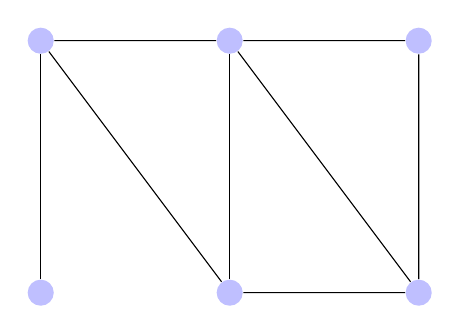
\begin{tikzpicture}
[scale=.8,auto=left,every node/.style={circle,fill=blue!25}]
  \node (n6) at (3,2) {};
  \node (n4) at (3,6) {};
  \node (n5) at (6,2) {};
  \node (n1) at (6,6) {};
  \node (n2) at (9,2) {};
  \node (n3) at (9,6) {};
  \foreach \from/\to in {n6/n4,n4/n5,n5/n1,n1/n2,n2/n5,n2/n3,n3/n1,n1/n4}
    \draw (\from) -- (\to);
\end{tikzpicture}
\caption{Et eksempel på en simpel, endelig graf} \label{simpel_graf}
\end{figure}


\noindent I figur \ref{simpel_graf} er skitseret en simpel graf med $6$ knuder og $8$ forbindende kanter. \\ 

\noindent Optræder der et uordnet punktpar ${u,v}$ i grafen, som forbindes af to eller flere kanter, kaldes grafen en \textit{multigraf}, og findes der et punkt i grafen, som via en kant forbindes med sig selv (en \textit{løkke}), er der tale om en \textit{pseudograf}.

\begin{figure}[h]
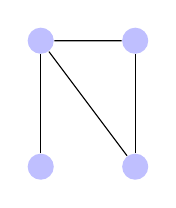
\begin{tikzpicture}
[scale=.4,auto=left,every node/.style={circle,fill=blue!25}]
  \node (n6) at (3,2) {};
  \node (n4) at (3,6) {};
  \node (n5) at (6,2) {};
  \node (n1) at (6,6) {};
  \foreach \from/\to in {n6/n4,n4/n5,n5/n1,n1/n4}
    \draw (\from) -- (\to);
\end{tikzpicture}
\caption{Et eksempel på en simpel, endelig graf} \label{simpel_graf}
\end{figure}

\noindent Det kan imidlertid være nødendigt at give kanterne retning, for at indikere, hvilken retning forbindelsen mellem to punkter har. I grafer over eksempelvis trafikale netværk, kan det være nødvendigt at indikere, i hvilken retning, trafikken kører eller at angive ensrettede strækninger. Til disse formål vil en simpel graf være utilstrækkelig idet kanterne deri netop ingen bestemt retning har. Derfor anledes definition \ref{def_retn_graf} 
af en \textit{retningsbestemt graf}:

\begin{defn}
En retningsbestemt graf $G = (V, E)$ består af et antal knuder, $V$, og et antal \textit{retningsbestemte} kanter hvorom der gælder, at $V, E \neq \emptyset$.\\
En retningsbestemt kant $(u,v)$ forbinder et knudepar, så at kanten starter i $u$ og ender i $v$.
\label{def_retn_graf}
\end{defn} 

\noindent Denne definition (\ref{def_retn_graf}) tillader ydermere muligheden for, at et knudepar kan forbindes af indtil flere retningsbestemte kanter. Findes dette i grafen, kaldes den en \textit{retningsbestemt multigraf}, og denne må også indeholde løkker. I det tilfælde, at alle knudepar kun forbindes af netop én retningsbestemt kant er grafen en \textit{simpel retningsbestemt graf}.

\begin{figure}
\centering
	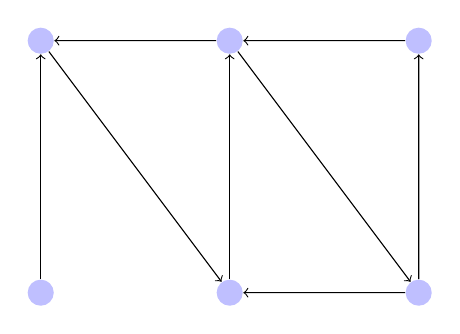
\begin{tikzpicture}
	[scale=.8,auto=left,every node/.style={circle,fill=blue!25}]
  \node (n6) at (3,2) {};
  \node (n4) at (3,6) {};
  \node (n5) at (6,2) {};
  \node (n1) at (6,6) {};
  \node (n2) at (9,2) {};
  \node (n3) at (9,6) {};
  \foreach \from/\to in {n6/n4,n4/n5,n5/n1,n1/n2,n2/n5,n2/n3,n3/n1,n1/n4}
    \draw [->] (\from) -- (\to);
	\end{tikzpicture}
\caption{Et eksempel på en retningsbestemt graf, hvor man kan se pilene definere retningen}
\end{figure}

\begin{figure}[h]
\centering
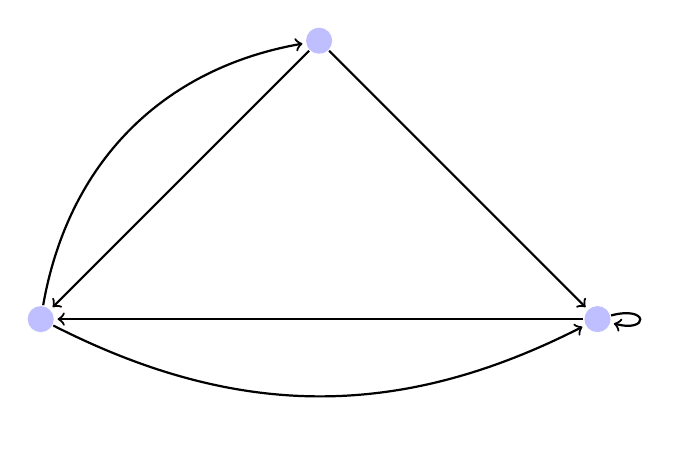
\begin{tikzpicture}[->,shorten >=1pt,auto,node distance=5cm,
                thick,main node/.style={circle,fill=blue!25}]

  \node[main node] (a) {};
  \node[main node] (b) [below left of=a] {};
  \node[main node] (c) [below right of=a] {};

  \path
    (a) edge node {} (b)
        edge node {} (c)
    (b) edge [bend left=35] node {} (a)
        edge [bend right=27] node {} (c)
    (c) edge [loop right] node {} (c)
        edge node [above] {} (b);
\end{tikzpicture}
\caption{•}
\end{figure}

\begin{table}
\begin{tabular}{|c|c|c|c|}
\hline 
Type & Kanter & Flerdobbelte kanter tilladt & Løkker \\ 
\hline
Simpel graf & Ikke-orienteret & Nej & Nej	 \\ 

Multigraf & Ikke-orienteret & Ja & Nej \\ 

Pseudograf & Ikke-orienteret & Ja & Ja \\ 
 
Simpel orienteret graf & Orienteret & Nej & Nej \\ 
 
Orienteret multigraf & Orienteret & Ja & Ja \\ 
 
Kombineret graf & Orienteret og ikke-orienteret & Ja & Ja \\ 
\hline 
\end{tabular}
\caption{bla} \label{table:graf_oversigt}
\end{table}

\usetikzlibrary{arrows, positioning}
\section{Grafer 2}
\subsection{Grafterminologi}

Der findes begreber til at beskrive kanter og knuder i ikke-orienterede grafer, som bl.a. beskriver hvordan knuder og kanter er orienterede i forhold til hinanden samt hvor mange knuder eller kanter, der er forbundet til en given knude.

\begin{defn}
To knuder $u$ og $v$ siges at være naboer i en ikke-orienteret graf $G$, hvis $u$ og $v$ er endepunkter i en kant $e$. Desuden siges kanten $e$ at forbinde $u$ og $v$, og $e$ er incident med både $u$ og $v$.
\end{defn}

\begin{defn}
En mængde af alle naboer til en knude $v$ i en graf $G=(V,E)$ betegnes $N(v)$ og kaldes et nabolag af $v$. Hvis $A$ er en delmængde af $V$, betegner $N(A)$ mængden af alle knuder i $G$, som er nabo til mindst én knude i $A$.
\end{defn}

\begin{defn}
Graden af en knude i en ikke-orienteret graf betegnes $deg(v)$ og er antallet af kanter incidente med den givne knude.  Et muligt loop vil bidrage med to grader til knuden. 
\end{defn}

En knude med grad 0 betegnes som værende \textit{isoleret} og har ingen incidente kanter. En knude med grad 1 betegnes som et \textit{vedhæng} og har netop én incident kant.

\begin{exmp}
Bestem graden af knuderne og nabolagene for knuderne i grafen i figur \ref{eksempel_nabo} og identificer isolerede knuder eller vedhæng.\\
Graden af en knude i grafen i figur \ref{eksempel_nabo} bestemmes ved at identificere antal incidente kanter til knuden. Derfor er $deg(A)=1$, $deg(B)=3$, $deg(C)=3$, $deg(D)=4$, $deg(E)=3$ og $deg(F)=2$. 
Nabolagene for de enkelte knuder er mængden af naboknuder. 
Derfor er $N(A)=\lbrace B \rbrace$, $N(B)=\lbrace A, C, D \rbrace$, $N(C)=\lbrace B, D, E \rbrace$, $N(D)=\lbrace B, C, E, F \rbrace$, $N(E)=\lbrace C, D, F \rbrace$ og $N(F)=\lbrace D, E \rbrace$. 
I grafen er A et vedhæng, og der forefindes ingen isolerede knuder.
\end{exmp}

\begin{figure}[h]
\centering
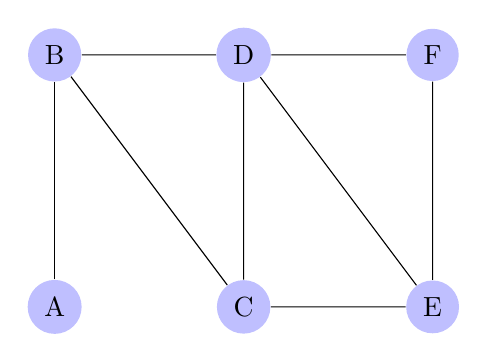
\begin{tikzpicture}
[scale=.8,auto=left,every node/.style={circle,fill=blue!25}]
  \node (n6) at (3,2) {A};
  \node (n4) at (3,6) {B};
  \node (n5) at (6,2) {C};
  \node (n1) at (6,6) {D};
  \node (n2) at (9,2) {E};
  \node (n3) at (9,6) {F};
  \foreach \from/\to in {n6/n4,n4/n5,n5/n1,n1/n2,n2/n5,n2/n3,n3/n1,n1/n4}
    \draw (\from) -- (\to);
\end{tikzpicture}
\caption{Simpel ikke-orienteret graf} \label{eksempel_nabo}
\end{figure}

For at beskrive summen af graderne for alle knuder i en graf anvendes \textit{The Handshaking Theorem}. 

\begin{thm}\label{handshake}
\textbf{The Handshaking Theorem}. Lad $G=(V,E)$ være en ikke-orienteret graf med $m$ kanter. Så er summen af knudernes grader \\
\begin{align*}
2m=\sum_{v \in V}deg(v)
\end{align*}
\end{thm}

\begin{proof}
I en ikke-orienteret graf med $m$ kanter, bidrager hver kant i en graf med to grader - én grad til hvert endepunkt. Det samlede antal grader for alle knuder i en graf stiger således med to pr. kant og summen af $deg(v)$ er $2m$. 
\end{proof}

Som følge af \ref{handshake} er summen af knudernes grader et lige tal. Derfor har en ikke-orienteret graf et lige antal knuder, hvor graden er et ulige tal.

\begin{thm}
En ikke-orienteret graf har et lige antal knuder af ulige grad. 
\end{thm}

\begin{proof}
Lad $V_1$ og $V_2$ være henholdsvis mængden af knuder af lige grad og mængden af knuder af ulige grad i en ikke-orienteret graf $G=(V,E)$ med $m$ kanter. Så er \\
\begin{align*}
2m=\sum_{v \in V}deg(v)=\sum_{v \in V_1}deg(v)+ \sum_{v \in V_2}deg(v)
\end{align*}
Da $deg(v)$ er lige for $v \in V_1$, er summen $\sum_{v \in V_1}deg(v)$ også lige. Summen af de to led på højresiden i ligningen er lige, fordi de tilsammen er lig $2m$, hvorfor $\sum_{v \in V_2}deg(v)$ også er lige. Summen $\sum_{v \in V_2}deg(v)$ består af en række ulige tal, og for at summen bliver lige, skal der således være et lige antal ulige led i summen.
Idet summen af graderne for knuderne af ulige grad i grafen er lige, må der være et lige antal af sådanne knuder.
\end{proof}




\subsection{Repræsentation af grafer}

Der er flere brugbare måder at repræsentere grafer på, og man ønsker i hvert tilfælde at vælge den pæneste repræsentation. \\
En overskuelig måde at repræsentere en graf på er ved matricer. To matricer, der almindeligvis bruges, er nabo-matricer, der er baseret på nabo-knuder, og incidens-matricer baseret på incidensen af knuder og kanter. \\
Antag at $G=(V,E)$ er en simpel graf med $n$ knuder, hvor knuderne i $G$ står skrevet i vilkårlig rækkefølge som $v_1$, $v_2$, \dots , $v_n$. Nabo-matricen $A$  af G er en $n \times n$ nul-et matrix, med 1 som den $(i,j)$’te indgang når $v_i$ og $v_j$ er naboer, og 0 er den $(i,j)$’te indgang, når de ikke er naboer. Hvis nabo-matricen er $A=[a_{ij}]$ så er

\begin{align*}
a_{ij}= \left\{\begin{array}{cc}
1 & \textrm{hvis} \  \lbrace v_i, v_j \rbrace \  \textrm{er} \  \textrm{en} \  \textrm{kant} \  \textrm{i} \  G \\
0 & \textrm{ellers} \\
\end{array}\right.
.
\end{align*}

En nabo-matrix af en graf er baseret på den valgte ordning af knuderne, hvorfor der kan være $n!$ forskellige nabo-matricer for en graf med $n$ knuder, idet der er $n!$ forskellige måder at ordne de $n$ knuder. Nabo-matricen for en simpel graf er symmetrisk dvs. $a_{ij}=a_{ji}$, da begge indgange er 1, når de relaterede knuder er naboer, og 0 hvis de ikke er. Da en simpel graf ikke består af loops, er hver indgang $a_{ii},i=1,2,3, \dots ,n$ $0$. \\
Nabo-matricer kan også bruges til at repræsentere ikke-orienterede grafer med loops og flere kanter til samme knuder. Et loop ved en knude $v_i$ er repræsenteret ved 1 ved position $(i,i)$ i nabo-matricen. Når flere kanter forbinder det samme par af knuder $v_i$ og $v_j$, eller der er flere loops ved samme knude til stede, er nabo-matricen ikke længere en nul-et matrix, i det den $(i,j)$’te indgang af matricen er lig antallet af kanter forbundet til ${v_i,v_j}$. Alle ikke-orienterede grafer, herunder multi- og pseudografer, har symmetriske nabo-matricer. 

 \begin{equation*}
  \mathbf{A}=
  \begin{blockarray}{*{6}{c} l}
    \begin{block}{*{6}{>{$\footnotesize}c<{$}} l}
      A & B & C & D & E & F \\
    \end{block}
    \begin{block}{[*{6}{c}]>{$\footnotesize}l<{$}}
      0 & 1 & 0 & 0 & 0 & 0 \bigstrut[t]& A \\
      1 & 0 & 1 & 1 & 0 & 0 \bigstrut[t]&B \\
      0 & 1 & 0 & 1 & 1 & 0 \bigstrut[t]&C \\
      0 & 1 & 1 & 0 & 1 & 1 \bigstrut[t]& D \\
      0 & 0 & 1 & 1 & 0 & 1 \bigstrut[t]& E \\
      0 & 0 & 0 & 1 & 1 & 0 \bigstrut[t]& F \\
    \end{block}
  \end{blockarray}
\end{equation*}

\noindent En anden almindelig måde at repræsentere grafer på er ved incidens-matricer. Lad $G=(V,E)$ være en ikke-orienteret graf med knuderne $v_1$, $v_2$, \dots , $v_n$ og kanterne $e_1$, $e_2$, \dots , $e_n$. Incidens-matricen, i forhold til ordningen af $V$ og $E$, er en $n x m$ matrix $M=[m_{ij}]$, hvor 
\begin{align*}
m_{ij}= \left\{\begin{array}{cc}
1 & \textrm{hvis} \  {e_j} \  \textrm{er} \  \textrm{nabo} \ \textrm{til} \ v_i \\
0 & \textrm{ellers} \\
\end{array}\right.
\end{align*}

\noindent Incidensmatricer kan også bruges til at repræsentere flere kanter og løkker. Flere kanter ved én knude er repræsenteret i incidens-matricen ved kolonner med identiske indgange, idet disse kanter er incidente med det samme knudepar. Løkker er repræsenteret ved en kolonne med præcis én indgang lig 1, der svarer til den knude, der er incident med løkken. 

 \begin{equation*}
  \mathbf{M}=
  \begin{blockarray}{*{8}{c} l}
    \begin{block}{*{8}{>{$\footnotesize}c<{$}} l}
      1 & 2 & 3 & 4 & 5 & 6 & 7 & 8 \\
    \end{block}
    \begin{block}{[*{8}{c}]>{$\footnotesize}l<{$}}
      1 & 0 & 0 & 0 & 0 & 0 & 0 & 0 \bigstrut[t]& A \\
      1 & 1 & 1 & 0 & 0 & 0 & 0 & 0 \bigstrut[t]&B \\
      0 & 1 & 0 & 1 & 1 & 0 & 0 & 0 \bigstrut[t]&C \\
     0 & 0 & 1 & 1 & 0 & 1 & 1 & 0 \bigstrut[t]& D \\
      0 & 0 & 0 & 0 & 1 & 1 & 0 & 1 \bigstrut[t]& E \\
     0 & 0 & 0 & 0 & 0 & 0 & 1 & 1 \bigstrut[t]& F \\
    \end{block}
  \end{blockarray}
\end{equation*}


\begin{figure}[!h]
  \centering
  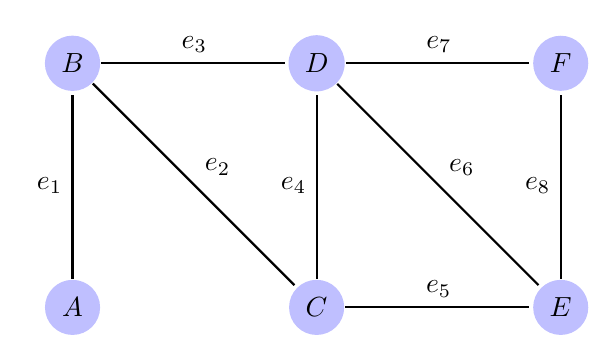
\begin{tikzpicture}
  [shorten >=1pt,node distance=3.1cm,on grid,auto]
    \tikzstyle{state}=[shape=circle,fill=blue!25,thick,minimum size=0.7cm]

    \node[state] (A) {$A$};
    \node[state,above of=A] (B) {$B$};
    \node[state,right of=A] (C) {$C$};
    \node[state,right of=B] (D) {$D$};
    \node[state,right of=C] (E) {$E$};
    \node[state,right of=D] (F) {$F$};

    \path[-,draw,thick]
    (A) edge node {$e_1$} (B)
    (B) edge node {$e_2$} (C)
    (B) edge node {$e_3$} (D)
    (C) edge node {$e_4$} (D)
    (C) edge node {$e_5$} (E)
    (D) edge node {$e_6$} (E)
    (D) edge node {$e_7$} (F)
    (E) edge node {$e_8$} (F)
    ;
  \end{tikzpicture}
  \caption{Model}
  \label{fig:f1}
\end{figure}





\section{Komplette grafer}
En komplet graf er en graf hvor et hvert unikt par af knuder i grafen er forbundet.
En komplet graf navngives $K_n$ hvor $n$ er antallet af knuderf i grafen.
I figur \ref{fig:komplette_grafer} ses de første 5 komplette grafer.
En graf hvor mindst ét par af knuder ikke er forbundet, kaldes en ikke-komplet graf.

\begin{figure}[h]
	\centering
	% Radius of regular polygons
\newdimen\R
\R=1cm

\begin{tikzpicture}[thick]
  \foreach \x in {1,2,3,4,5}{
    \node[yshift=-1.5\R, xshift=\x*2.5\R-2.5\R] {$K_\x $} {};
  }
  \begin{scope}[every node/.style={circle,fill=blue!25}]
    \node (0:0) {};

    \foreach \x in {1,2}{
      \node[xshift=2.5\R] (\x) at (\x*180-180:\R) {};
    }
    \path (1) edge (2);

    \foreach \x in {1,2,3}{
      \node[xshift=5\R] (\x) at (\x*120-120:\R) {};
    }
    \path (1) edge (2);
    \path (2) edge (3);
    \path (3) edge (1);
  
    \foreach \x in {1,2,3,4}{
      \node[xshift=7.5\R] (\x) at (\x*90-90:\R) {};
    }
    \foreach \x in {1,2,3}{
      \path (4) edge (\x);
    }
    \foreach \x in {1,2}{
      \path (3) edge (\x);
    }
    \path (1) edge (2);
  
    \foreach \x in {1,2,3,4,5}{
      \node[xshift=10\R] (\x) at (\x*72-72:\R) {};
    }
    \foreach \x in {1,2,3,4}{
      \path (5) edge (\x);
    }
    \foreach \x in {1,2,3}{
      \path (4) edge (\x);
    }
    \foreach \x in {1,2}{
      \path (3) edge (\x);
    }
    \path (1) edge (2);
  \end{scope}
\end{tikzpicture}

	\caption{De første $5$ komplette grafer} \label{fig:komplette_grafer}
\end{figure}

Antallet af kanter i en komplet graf $K_n$ afhænger kun af $n$.

\begin{thm}
	For en komplet graf $K_n = (V_n, E_n)$ med $n$ knuder er $|E_n|$ antallet af kanter. Da er
	\begin{align*}
		|E_n| = \frac{n (n - 1)}{2}
	\end{align*}
\end{thm}
\begin{proof}
	For at gennemføre et induktionsbevis skal basisskridtet og induktionsskridtet gennemføres.
	Lad propositionen $P(n)$ være at $|E_n|= \frac{n (n - 1)}{2}$, hvor $n$ er antal knuder i en komplet graf $K_n$ og $m$ være antal kanter.

	\textit{Basisskridt:} $K_1$ består af en enkelt knude, og da der ikke er et par af knuder i grafen, må der da ikke eksistere nogen kanter.
	$\frac{ 1 \cdot 0}{2} = 0$, hvilket betyder at $P(1)$ er sand. Da er basisskidtet gennemført.

	\textit{Induktionsskridt:} Det skal nu vises at der for et vilkårligt $k$ gælder at $P(k) \to P(k + 1)$, altså at $|E_k| = \frac{k (k - 1)}{2}$ medfører at $|E_{k+1}| = \frac{k (k + 1)}{2}$.

	Antag at $|E_k| = \frac{k (k - 1)}{2}$ for $K_k$.
	Den næste komplette graf $K_{k+1}$ må være den graf hvor der er én til knude. Denne nye knude $v$ skal være forbundet til alle knuder i $K_k$ for at være en komplet graf. $\deg (v)$ må da være lig $k$. Da må
	\begin{align*}
		|E_{k+1}| 
		&= |E_k| + k \\
		&= \frac{k (k - 1)}{2} + k \\
		&= \frac{k^2 - k}{2} + \frac{2k}{2} \\
		&= \frac{k^2 + k}{2} \\
		&= \frac{k (k + 1)}{2}
	\end{align*}
	Dette er netop $P(k + 1)$, hvilket betyder at induktionsskridtet er gennemført.
\end{proof}


\chapter{Veje og Kredse}

\section{Veje}
Veje i en graf viser, hvilke ruter der er rundt i en graf. Dette er relevant for at finde ruter til en GPS, et computernetværk eller andet, hvor der er behov for at bestemme en rute gennem flere steder. 
En vej i en graf defineres i Definition \ref{def_vej}.

\begin{defn} \label{def_vej}
	Lad $n \in  \mathbb{Z}^{+}$ og lad $G$ være en ikke-orienteret graf. 
	En \textit{vej} af \textit{længde} $n$ fra $v_0$ til $v_n$ i $G$ er en sekvens af $n$ kanter $e_1, ..., e_n$ i $G$, for hvilke der eksisterer en sekvens $v_0,v_1,...,v_{n-1},v_n$ af knuder, så $e_i$ har endeknuderne $v_{i-1}$ og $v_i$ for $i=1,...,n$.
\end{defn}

Når der er tale om en vej gennem en simpel graf, angives denne som sekvensen af de knuder, den går igennem $v_0, v_1,...,v_n$. 
En vej er \textit{simpel} hvis den ikke indeholder den samme kant mere end én gang. 

\begin{exmp} \label{ex_vej}
	På den simple graf i Figur \ref{graf_vej} ses en simpel vej $A,B,E,F$ af længden 3, fordi vejen går gennem de tre kanter $\lbrace A,B \rbrace$, $\lbrace B,E \rbrace$ og $\lbrace E,F \rbrace$. 
	Vejen er simpel, fordi den ikke går gennem den samme kant mere end en gang. 
	Derimod er $A,B,D,E$ ikke en vej, fordi $\lbrace B,D \rbrace$ ikke er en kant. 
	Vejen $A,B,C,E,B,A$ er også en vej, men den er ikke simpel, fordi den går gennem kanten $\lbrace A,B \rbrace$ to gange. 
\end{exmp}

\begin{figure}[h]
	\centering
	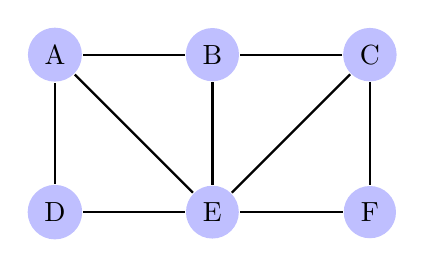
\begin{tikzpicture}
[auto,thick,node distance=2cm,every node/.style={circle,fill=blue!25}]
  \node (n6) {D};
  \node (n4) [above of=n6] {A};
  \node (n5) [right of=n6] {E};
  \node (n1) [right of=n4] {B};
  \node (n2) [right of=n5] {F};
  \node (n3) [right of=n1] {C};
  \foreach \from/\to in {n6/n4,n4/n5,n5/n1,n2/n5,n2/n3,n3/n1,n1/n4,n6/n5,n5/n3}
    \draw (\from) -- (\to);
\end{tikzpicture}

	\caption{Et eksempel på en simpel graf, hvor der indgår simple veje.} \label{graf_vej}
\end{figure}

\section{Kredse}
I et særligt tilfælde kan en vej kaldes en kreds.
En kreds er en vej, der starter og slutter det samme sted, hvilket defineres i Definition \ref{def_kredse}

\begin{defn}
\label{def_kredse}
En vej kaldes en \textit{kreds}, hvis den begynder og ender i samme knude $v_0=v_n$, og $n>0$.
Kredsen siges at gå gennem knuderne $v_0,v_1,...,v_{n-1}$ eller passere gennem kanterne $e_1, e_2,..., e_n$.
\end{defn}

\begin{exmp}
I Figur \ref{graf_kreds} ses en kreds, $A,B,C,E,D,A$, som har længden 5, fordi den går gennem 5 kanter. Det er en kreds, fordi den begynder og ender i knuden $A$.
I Figur \ref{graf_ikke_kreds} ses en vej $C,B,A,D,E,C,F$.
Denne vej er ikke en kreds, fordi den ikke starter og slutter i samme knude. 
\end{exmp}

\begin{figure}[!htb]
   \begin{minipage}{0.48\textwidth}
     \centering
		 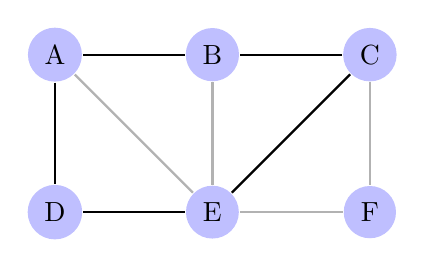
\begin{tikzpicture}
[auto,thick,node distance=2cm,every node/.style={circle,fill=blue!25}]
  \node (D) {D};
  \node (A) [above of=D] {A};
  \node (E) [right of=D] {E};
  \node (B) [right of=A] {B};
  \node (F) [right of=E] {F};
  \node (C) [right of=B] {C};

	\path
	(C) edge (B) (B) edge (A) (A) edge (D) (D) edge (E) (E) edge (C);
	\path[black!30]
	(E) edge (A)
			edge (B)
	(F) edge (C)
			edge (E);

\end{tikzpicture}

     \caption{Et eksempel på en kreds i en simpel graf.}
     \label{graf_kreds}
   \end{minipage}\hfill
   \begin{minipage}{0.48\textwidth}
     \centering
		 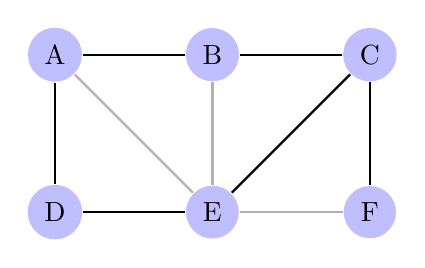
\begin{tikzpicture}
[auto,thick,node distance=2cm,every node/.style={circle,fill=blue!25}]
	\node (D) {D};
  \node (A) [above of=D] {A};
  \node (E) [right of=D] {E};
  \node (B) [right of=A] {B};
  \node (F) [right of=E] {F};
  \node (C) [right of=B] {C};

	\path
	(F) edge (C) (C) edge (B) (B) edge (A) (A) edge (D) (D) edge (E) (E) edge (C);

	\path[black!30]
	(E) edge (A)
	    edge (B)
	(F) edge (E);
\end{tikzpicture}

     \caption{Et eksempel på en vej i en simpel graf.}
     \label{graf_ikke_kreds}
   \end{minipage}
\end{figure}

\section{Sammenhængende grafer}
For en graf kan det være relevant at afgøre, om der er en vej mellem alle knuder i grafen, således, at det er muligt at komme fra en hvilken som helst knude til en anden.
I dette kapitel vil der kun blive fokuseret på ikke-orienterede grafer.

\begin{defn}
\label{def_iosmh}
En graf siges at være \textit{sammenhængende}, hvis der er en vej mellem hvert knudepar i grafen. 
\end{defn}


\begin{thm}
Der er en simpel vej mellem ethvert knudepar i en sammenhængende graf.
\label{smh_satning}
\end{thm}

\begin{proof}
Lad knuderne $u$ og $v$ være to knuder i den sammenhængende graf $G=(V,E)$.
Per Definition \ref{def_iosmh} er der en vej mellem $u$ og $v$.
Lad en kortest mulig vej mellem $u$ og $v$ være $v_0,v_1,...,v_n$, hvor $v_0=u$ og $v_n=v$.

For modstrid antages det, at denne vej ikke er simpel. 
Så er $v_i=v_j$ for $0 \leq i < j$, fordi vejen går gennem kanten $v_i,v_{i+1}$ to gange, specielt besøges $v_i$ to gange.
Det betyder, at der er en kortere vej fra $u$ til $v$, med knudesekvens $v_0,v_1,...,v_{i-1},v_j,...,v_n$, som opnåes ved at fjerne kanterne i sekvensen $v_i,...,v_{j-1}$.
Dette er i modstrid med antagelsen om, at vejen var kortest mulig.
Det må derfor gælde, at der er en simpel vej mellem alle knudepar i en sammenhængende graf. 
\end{proof}

Flere problemstillinger kan modelleres ved brug af grafer med vægte tildelt kanterne. 
Det kan f.eks. være distance, den samlede rejsetid, eller billetprisen for at rejse mellem to byer. 
Grafer, der har vægte tildelt kanterne, kaldes vægtede grafer. 
Der opstår jævnligt forskellige typer af problemer, der involverer vægtede grafer, hvor en korteste rute, mellem to knuder i et netværk, skal bestemmes. 
Længden af en vej i en graf uden vægte er tidligere betegnet ved antallet af kanter, vejen går igennem.
I en vægtet graf er længden af vejen summen af alle kanternes vægte, der indgår i vejen. 
Et interessant problem, som involverer vægtede grafer, søger en kreds af kortest mulig totallængde, der besøger hver knude i en komplet graf præcis én gang.
Der er her tale om \emph{traveling salesperson problem}, som søger dén rækkefølge, knuderne skal besøges i, som resulterer i en kreds af kortest mulig længde. 

\section{Eulerkredse og -veje}

En bestemt type af kredse gennemgår alle kanter i en graf og kaldes Eulerkredse. 

\begin{defn}\label{euler_def}
	En Eulerkreds er en simpel kreds i grafen $G$ som indeholder hver kant i $G$.
	En Eulervej er en simpel vej i grafen $G$, som indeholder hver kant i $G$.  
\end{defn}

\begin{exmp}
	Et eksempel på en Eulerkreds og en Eulervej kan ses i Figur \ref{euler_kreds} og \ref{euler_vej}: 
\end{exmp}

\begin{figure}[h]
\centering
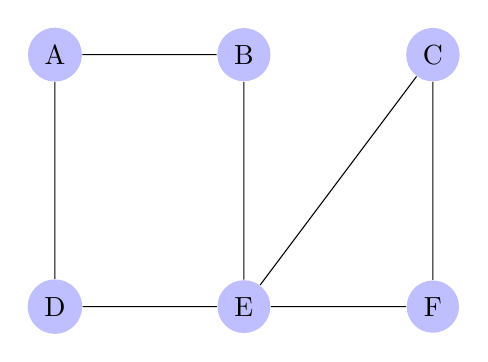
\begin{tikzpicture}
[scale=.8,auto=left,every node/.style={circle,fill=blue!25}]
  \node (n6) at (3,2) {D};
  \node (n4) at (3,6) {A};
  \node (n5) at (6,2) {E};
  \node (n1) at (6,6) {B};
  \node (n2) at (9,2) {F};
  \node (n3) at (9,6) {C};
  \foreach \from/\to in {n6/n4,n5/n1,n2/n5,n2/n3,n1/n4,n6/n5,n5/n3}
    \draw (\from) -- (\to);
\end{tikzpicture}
\caption{Euler kreds} 
\label{euler_kreds}
\end{figure}

\begin{figure}[h]
\centering
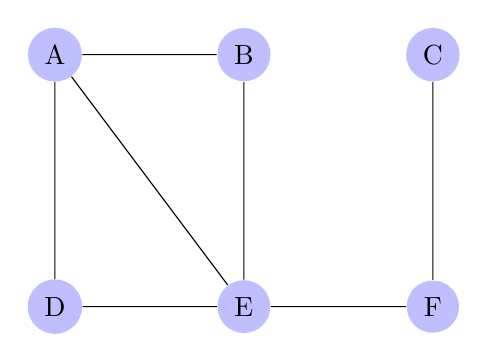
\begin{tikzpicture}
[scale=.8,auto=left,every node/.style={circle,fill=blue!25}]
  \node (n6) at (3,2) {D};
  \node (n4) at (3,6) {A};
  \node (n5) at (6,2) {E};
  \node (n1) at (6,6) {B};
  \node (n2) at (9,2) {F};
  \node (n3) at (9,6) {C};
  \foreach \from/\to in {n6/n4,n5/n1,n2/n5,n2/n3,n1/n4,n6/n5,n4/n5}
    \draw (\from) -- (\to);
\end{tikzpicture}
\caption{Euler vej} 
\label{euler_vej}
\end{figure}

Et eksempel på en Eulerkreds i Figur \ref{euler_kreds} kan være: $A,B,E,C,F,E,D,A$, og
et eksempel på en Eulervej i Figur \ref{euler_vej} kan være: $A,B,E,D,A,E,F,C$.

Der eksiserer ikke en Eulerkreds i alle grafer.

\begin{thm}\label{Eulerkreds_multigraf}
	En sammenhængende multigraf med mindst to knuder, har en Eulerkreds hvis og kun hvis, hver knude er af lige grad.
\end{thm}

\begin{proof} 
	Først bevises det at hvis en graf har en Eulerkreds, så er graden af alle knuderne i grafen lige. 

	En kreds begynder i en knude $a$ og fortsætter langs en kant, som er incident med $a$, til en ny knude $b$. 
	Denne kant bidrager med 1 til $\deg(a)$. 
	Hver gang kredsen passerer gennem en knude, tilføjes 2 til graden af denne knude. 
	Til sidst ender kredsen tilbage i $a$, og bidrager igen med 1 til $\deg(a)$.
	Hele graden af hver knude opnåes, da alle kanter skal passeres.  
	Derfor må $\deg(a)$ være lige og graden af hver knude må også være lige.  
	
	Nu bevises at hvis alle knuder er af lige grad, vil der eksistere en Eulerkreds i grafen.

	For at finde en Eulerkreds i en sammenhægende multigraf  $G$, som opfylder at graden af hver knude er lige, tages først udgangspunkt i en tilfældig underkreds i $G$.
	Denne underkreds starter i en knude $a$, hvorfra en simpel vej dannes ved at bevæge sig rundt i grafen. 
	Dette forsættes indtil en knude nås, hvorfra det ikke er muligt at komme videre, fordi alle incidente kanter allerede er en del af den simple vej.
	Denne knude må være knuden $a$. 
	Da alle knuder er af lige grad, vil det være muligt at komme ud af en hvilken som helst anden knude end $a$, som vejen passerer. 
	Vejen må nu være blevet til en kreds.  
	Herefter indførers $H$, som er lig med $G$, frataget kanterne i den tilfældige underkreds.
	Alle knuder i grafen vil stadig være af lige grad.
	Så dannes en ny underkreds i $H$, som starter i et endepunkt i den tidligere underkreds.
	Fordi grafen er sammenhængende vides det at den nye underkreds kan startes i en knude i den tidligere underkreds. 
	Kanter i den nye underkreds fjernes fra $H$. 
	Samtidig sættes de to underkredse sammen til én kreds.
	Denne procedure forsættes, indtil der ikke er flere kanter i $H$.
	Da må der være dannet en Eulerkreds. 
\end{proof} 
 
Proceduren kan ses i Algoritme \ref{algoritme_euler}.
Der findes også andre algoritmer, som kan finde Eulerkredse i en graf, men disse bliver ikke nævnt i dette projekt.
  
\begin{algorithm}
	\caption{Eulerkredse}
	\label{algoritme_euler}
	\textbf{procedure} Euler(G: sammenhængende multigraf med knuder af lige grad)\\
	$kreds:=$ en kreds i G der begynder i en vilkårlig knude med kanter, der danner en kreds.\\
	$H:= G$ med kanterne fra $kreds$ fjernet\\
	\textbf{så længe} $H$ har kanter\\
	$\-$ $\-$ $\-$ $\-$ $\-$ $\-$
	$underkreds:=$ en kreds i $H$, der begynder i en knude $v$ i $H$, som også er et endepunkt af en kant i $kreds$ \\ 
	$\-$ $\-$ $\-$ $\-$ $\-$ $\-$
	$H:=$ $H$ uden kanterne af $underkreds$ samt alle isolerede knuder fjernet \\
	$\-$ $\-$ $\-$ $\-$ $\-$ $\-$
	$kreds:=$ $kreds$ med $underkreds$ indsat \\ 
	\textbf{retuner} $kreds$ ($kreds$ er en Eulerkreds)
\end{algorithm}

\begin{thm} \label{thm:O_euler}
	Kompleksiteten af Algoritme \ref{algoritme_euler} er af lineær orden.
\end{thm}

\begin{proof}
	For at finde algoritmens kompleksitet, opskrives en funktion, der beskriver antallet af sammenligner algoritmen laver for hver kant, $e$.
	Der tages udgangspunkt i det værst mulige tilfælde. 

	Hver gang algoritmen er ved en knude, vil den undersøge, om den kan vælge en kant, hvor den ikke allerede har været. 
	Dette kræver en sammenligning per kant.
	Finder algoritmen ved sammenligning, at den ikke kan vælge en kant, som den ikke har valgt før, vil den fjerne den underkreds der er dannet. 
	Dette gør, at algoritmen må tage udgangspunkt i en ny knude, som er incident med en af kanterne i den fjernede underkreds.
	I den nye knude vil algoritmen lave en ny sammenligning, for at finde ud af, om den kan vælge en kant, hvor den ikke har været før.
	Dette vil betyde, at det værst mulige tilfælde vil være i en multigraf, hvor der hele tiden vil blive dannet underkredse bestående af to kanter. 
	Hver gang algoritmen danner en ny underkreds, vil det kræve en ekstra sammenligning, og fordi dette sker hver anden gang i værste tilfælde, vil den endelige forskrift for antallet af sammenligninger blive $f(e)=e+ \frac{e}{2}$.

	Funktionen $f(e)$ er $O(e)$ da
	\begin{align*}
	e+ \frac{e}{2} \leq e + e = 2e
	\end{align*}
	når $e>1$. Da er vidnerne $C=2$ og $k=1$.

	Funktionen $f(n)$ er også $\Omega(e)$ da
	\begin{align*}
	e + \frac{e}{2} \geq e
	\end{align*}
	når $e>1$. Da er vidnerne $C=1$ og $k=1$.

	Da funtionen både er $O(e)$ og $\Omega (e)$ kan den også siges at være $\Theta (e)$.
\end{proof}

Hvis der ikke findes en Eulerkreds i en graf, kan der godt eksistere en Eulervej. 

\begin{thm} \label{Eulervej_multigraf}
	En sammenhængende multigraf graf $G$ har en Eulervej, men ikke en Eulerkreds, hvis og kun hvis den har præcist to knuder af ulige grad.  
\end{thm} 

\begin{proof}
	Først bevises det at hvis der eksisterer en Eulervej i en graf, vil netop to knuder være af ulige grad. 

	Antag at en sammenhængende multigraf, $G$, har en Eulervej fra $a$ til $b$, men ikke en Eulerkreds. 
	Den første kant som passeres på vejen bidrager med 1 til $\deg(a)$. 
	Hver gang vejen passerer knuden $a$ vil 2 tilføjes til $\deg(a)$. 
	Den sidste kant på vejen bidrager 1 til graden af endeknuden for vejen, $\deg(b)$. 
	Ligesom for $a$, kan vejen krydse $b$. 
	Hver gang dette måtte ske tilføjes 2 til graden af $b$. 
	Resultatet bliver, at $a$ og $b$ altid vil være af ulige grad. 
	Alle andre knuder på vejen vil være af lige grad, fordi 2 tilføjes til graden af en knude, hver gang en knude passeres.  
	
	Nu bevises det at hvis der indgår netop to knuder af ulige graf i grafen, vil der eksistere en Eulerkreds.

	Antag at $a$ og $b$ er de eneste knuder af ulige grad. 
	Hvis en kant $\lbrace a,b \rbrace$ tilføjes til $G$, vil alle knuder i grafen være af lige grad. 
	Så gælder Sætning \ref{Eulerkreds_multigraf}, og der vil være en Eulerkreds i $G$. 
	Fjernes kanten $\lbrace a,b \rbrace$ igen vil der være en Eulervej. 
\end{proof}

\section{Hamiltonkredse og -veje}
En anden type kreds er en Hamiltonkreds. 
En Hamiltonkreds er en kreds som går gennem hver knude i grafen én gang. På samme måde kan der også eksistere en Hamiltonvej, som er en vej der går gennem hver knude i en graf én gang. 

\begin{defn} \label{hamiltion_defn}
	En Hamiltonvej er en simpel vej i en graf $G$, som går gennem hver knude én gang.
	En simpel kreds i en graf $G$, som går gennem hver knude én gang kaldes en Hamiltonkreds.
\end{defn}

\begin{exmp}
	Eksempler på en Hamiltonkreds og en Hamiltonvej kan ses i Figur \ref{hamiltion_vej_kreds}.
	
	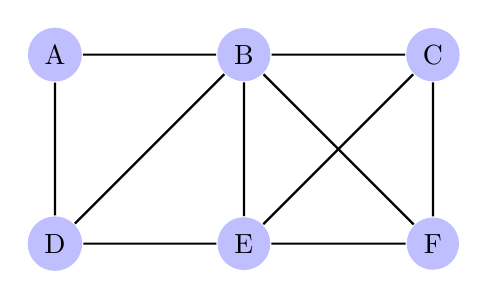
\begin{tikzpicture}
[thick,scale=.8,auto=left,every node/.style={circle,fill=blue!25}]
  \node (n6) at (3,2) {D};
  \node (n4) at (3,5) {A};
  \node (n5) at (6,2) {E};
  \node (n1) at (6,5) {B};
  \node (n2) at (9,2) {F};
  \node (n3) at (9,5) {C};
  \foreach \from/\to in {n6/n4,n4/n1,n6/n1,n6/n5,n1/n3,n1/n2,n1/n5,n5/n2,n5/n3,n3/n2}
    \draw (\from) -- (\to);
\end{tikzpicture}

	
	Et eksempel på en Hamiltonkreds i grafen er: $A,B,F,C,E,D,A$, og
	et eksempel på en Hamiltonvej er: $A,D,B,C,F,E$.
\end{exmp}

Der kendes ikke en simpel måde til at bestemme om der findes en Hamiltonkreds i en graf, ligesom der gør for en Eulerkreds. 
Der findes dog flere sætningerne der kan give en ide om eksistensen af en Hamiltonkreds. Med udgangspunkt i \citep{wilson_graph} og \citep{orebevis} bevises følgende to sætninger.

\begin{thm} \label{ores_thm}
	\textbf{Ores Sætning:} 
	Lad $G$ være er en simpel graf med $n$ knuder, og $n\geq3$, hvor $\deg(u)+\deg(v)\geq n$ for hvert par af knuder, $u$ og $v$, der ikke er naboer i $G$. 
	Da har $G$ en Hamiltonkreds. 
\end{thm}

\begin{proof}
	Lad $G=(V,E)$ være en graf med $n$ knuder, som opfylder sætningens betingelser. For modstrid antages det, at denne graf \textit{ikke} indeholder en Hamiltonkreds.

	Til denne graf kan der tilføjes kanter uden at overtræde sætningens betingelser. Antag nu, at grafen $G$ mangler netop én kant, for at indeholde en Hamiltonkreds. 
	Da må $G$ indeholde Hamiltonvejen 
	$$v_1, v_2,...,v_n,$$
	som går gennem alle grafens knuder. 
	Men idet $G$ ikke indeholder en Hamiltonkreds, må $v_1$ og $v_n$ da \textit{ikke} være naboer.
	Derfor opfylder de, at
	\begin{align} \label{eq:sum_deg}
		\textrm{deg}(v_1)+\textrm{deg}(v_n)\geq n.
	\end{align}

	Der må være en knude $v_i$ der er nabo til $v_1$, som opfylder, at $v_{i-1}$ er nabo til $v_n$.
	For at vise dette kan de følgende to mængder opstilles:
	\begin{align*}
		A &= \lbrace i: 2 \leq i \leq n-1, \; v_1 \; \textrm{er nabo til} \; v_i \rbrace \\
		B &= \lbrace i: 3 \leq i \leq n, \; v_n \; \textrm{er nabo til} \; v_{i-1} \rbrace,
	\end{align*}
	hvor $A$ er mængden af indekser på knuder, $v_1$ er nabo til, og $B$ er mængden af indekser plus 1, på knuder, $v_n$ er nabo til. 

	Om disse gælder, at
	\begin{align*}
		|A| &= \deg(v_1) \\
		|B| &= \deg(v_n),
	\end{align*}
	hvorfor $A,B \subseteq \lbrace 2,...,n \rbrace$, som indeholder $n-1$ elementer.
	Fra Ligning \eqref{eq:sum_deg} må $\deg(v_1) + \deg(v_n) \geq n$.
	Skuffeprincippet giver så, at $A$ og $B$ deler mindst ét element, og der må da findes et $v_i$ og et $v_{i-1}$ som er forbundet til henholdsvis $v_1$ og $v_n$.

	\begin{figure}[h!]
		\centering
		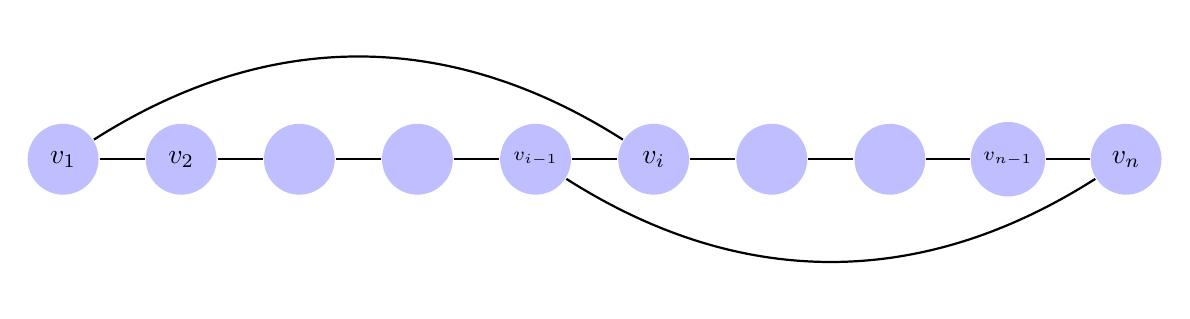
\begin{tikzpicture}                                         
[thick,auto,node distance=1.5cm,every node/.style={circle,minimum size=0.9cm,fill=blue!25}]
  \node (n1) {$v_1$};  
  \node (n2) [right of=n1] {$v_2$};
  \node (n3) [right of=n2] {};  
  \node (n4) [right of=n3] {};       
  \node (n5) [right of=n4] {\scriptsize $v_{i-1}$};
  \node (n6) [right of=n5] {$v_i$};
  \node (n7) [right of=n6] {}; 
  \node (n8) [right of=n7] {};         
  \node (n9) [right of=n8] {\scriptsize $v_{n-1}$};
  \node (n10) [right of=n9] {$v_n$};                                                
  \foreach \from/\to in {n1/n2,n2/n3,n3/n4,n4/n5,n5/n6,n6/n7,n7/n8,n8/n9,n9/n10}
    \draw (\from) -- (\to);
  \path                            
    (n1) edge [bend left=32.5] (n6)  
    (n10) edge [bend left=32.5] (n5);
\end{tikzpicture}

		\caption{En illustration der viser Hamiltonkredsen i $G$.} \label{ore_bevis}
	\end{figure}
	
	En Hamiltonkreds kan nu dannes af følgen $v_1, v_2,...v_{i-1},v_n,...,v_i,v_1$,
	som skitseres i Figur \ref{ore_bevis}. Dette er i modstrid med vores antagelse om, at der ikke eksisterer en Hamiltonkreds i en graf med de givne betingelser.	
\end{proof}

En anden sætning der kan bruges til at undersøge om der eksiserer en Hamiltonkreds i en graf er Diracs Sætning. 

\begin{thm} \label{diracs_thm}
	\textbf{Diracs Sætning:} 
	Lad $G$ være en simpel graf med $n$ knuder, og $n\geq3$, så graden af hver knude i $G$ er mindst $\frac{n}{2}$. Da har $G$ en Hamiltonkreds.  
\end{thm}

\begin{proof}
	Lad $G=(V,E)$ være en graf med 3 eller flere knuder. Udvælg fra grafen, $G$, to knuder, $u$ og $v$, der ikke er naboer. Det følger da direkte af Ores Sætning, at
	\begin{align*}
	\textrm{deg}(u) + \textrm{deg}(v) \geq \frac{n}{2} + \frac{n}{2} = n,
	\end{align*}
	hvorfor grafen må have en Hamiltonkreds.
\end{proof}

Derudover gælder det også, at der ikke kan eksistere en hamiltonkreds i en graf med en knude, der har graden 1. 
Disse to sætninger beskriver, hvornår der med sikkerhed eksisterer en Hamiltonkreds, men en Hamiltonkreds kan godt eksistere uden at opfylde sætningerne. 

\begin{exmp}
	I Figur \ref{pentagon} ses en graf der indeholder en hamiltonkreds.
	Grafen overholder ikke betingelserne i Ores' Sætning, da summen af to knuders grader aldrig kan give et resultat større end $4$, hvilket er mindre end $n$.
	Grafen overholder heller ikke betingelserne i Diracs Sætning, fordi $n=5$, mens graden af hver kant i grafen er $2$, hvilket er mindre end $n/2$.
	
	\begin{figure}[h]
	\centering
		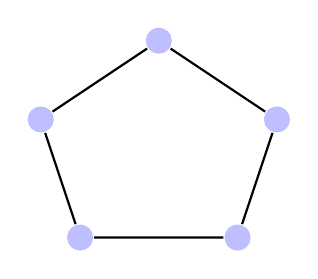
\begin{tikzpicture}[thick, every node/.style={shape=circle,fill=blue!25}]
	\path (0,0) node (p0) {}
	(-1.5,-1) node (p1) {}
	(-1,-2.5) node (p2) {}
	(1,-2.5) node (p3) {} 
	(1.5,-1) node (p4) {};
	\draw (p0) -- (p1)
	(p0) -- (p1)
	(p0) -- (p4)
	(p1) -- (p2)
	(p2) -- (p3) 
	(p3) -- (p4);    
\end{tikzpicture}                             

	\caption{Hamiltonkreds i en graf med 5 knuder}
	\label{pentagon}
	\end{figure}
\end{exmp}
%Et kendt probelm hedder...
%Der er blevet formuleret et problem, som kaldes Hamiltonvej Problemet eller Hamiltonkreds problemet. 
%Dette problem går ud på, at det ønskes at finde ud af om der eksisterer en hamiltonkreds eller -vej i en given graf. 

Problemet Hamiltonian Path Problem (HPP) er et kendt, svært problem inden for grafteori. 
Dette problem går netop ud på at finde ud af, om der eksisterer en hamiltonvej eller -kreds i en given graf.

\begin{thm} \label{HPP}
	Hamiltonian Path Problem er NP-fuldstændigt. \citep{computers}
\end{thm}

Der vil blive gjort brug af denne sætning i løbet af projektet, men denne vil ikke blive bevist. 
Der henvises til \citep{computers} for beviset.


\section{Træer}
\subsection{Terminologi for træer}

\begin{defn}
Et træ er en sammenhængende ikke-orienteret graf, der ikke indeholder en simpel kreds.
\label{def_tree}
\end{defn}

\noindent Træer er en type af simple grafer. Da de ikke indeholder en simpel kreds, kan der ikke være flere kanter mellem to knuder, og der kan ikke være løkker. Alternativt og ekvivalent til Definition \ref{def_tree} kan et træ defineres som følger.

\begin{thm}
En ikke-orienteret graf er et træ hvis og kun hvis, der eksistrerer netop én simpel vej mellem hvert par af knuder. 
\end{thm}

\begin{proof}
Antag at en ikke-orienteret graf $T$ er et træ, og lad $u$ og $v$ være to knuder i $T$. Da $T$ er sammenhængende må det betyde, at der er en simpel vej mellem $u$ og $v$ jf. Sætning \ref{smh_satning}. Den simple vej mellem $u$ og $v$ må være den eneste vej mellem $u$ og $v$, for hvis der eksisterer flere veje mellem $u$ og $v$, eksisterer en simpel kreds, for hvis der mellem $u$ og $v$ er to forskellige simple veje $P_{u,v}$ og $P_{v,u}$, må der være mindst ét punkt, der er forskelligt mellem de to veje. En simpel kreds opstår stedet mellem $u$ og $v$, hvor $P_{u,v}$ og $P_{v,u}$  er forskellige fra hinanden.  Eksistensen af en simpel kreds modstrider antagelsen om, at $T$ er et træ, og derfor må der være netop én simpel vej mellem hvert knudepar i $T$.

Antag nu, at der er netop én simpel vej mellem hvert knudepar i en ikke-orienteret graf $T$. Det betyder, at $T$ er sammenhængende. Desuden må det gælde, at $T$ ingen simple kredse har, da det vil stride i mod antagelsen om, at der er netop én simpel vej mellem hvert knudepar i en $T$. Der kan ikke eksistere en simpel kreds, der kun er én simpel vej mellem to knuder $u$ og $v$, og derfor kan der ikke findes punkter, hvor to eller flere veje mellem $u$ og $v$ er forskellige fra hianden, hvor der kan dannes en kreds. Grafen $T$ opfylder dermed kravene for at være et træ jf. Definition \ref{def_tree}.
\end{proof}

\begin{exmp}
For at illustrere en graf, som er et træ, og en graf, som ikke er et træ, iagttages hhv. Figur \ref{eksempel_tree} og Figur \ref{eksempel_notree}. Grafen i Figur \ref{eksempel_tree} er et træ, da det er en ikke-orienteret sammenhængende graf uden simple kredse.
\end{exmp}

\begin{figure}[h]
\centering
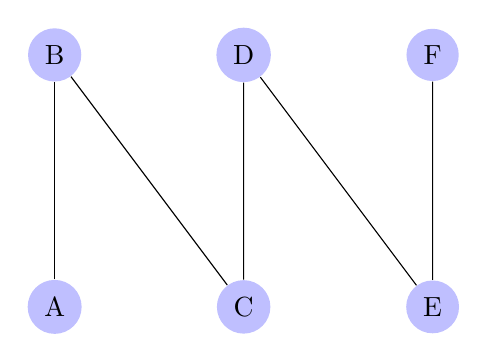
\begin{tikzpicture}
[scale=.8,auto=left,every node/.style={circle,fill=blue!25}]
  \node (n6) at (3,2) {A};
  \node (n4) at (3,6) {B};
  \node (n5) at (6,2) {C};
  \node (n1) at (6,6) {D};
  \node (n2) at (9,2) {E};
  \node (n3) at (9,6) {F};
  \foreach \from/\to in {n6/n4,n4/n5,n5/n1,n1/n2,n2/n3}
    \draw (\from) -- (\to);
\end{tikzpicture}
\caption{Et træ.} 
\label{eksempel_tree}
\end{figure}

\noindent Grafen i Figur \ref{eksempel_notree} er ikke et træ, da der eksistrer en kreds $\lbrace B, D, C \rbrace$. Grafen er heller ikke et træ med argumentet, at grafen ikke er sammenhængende.\\

\begin{figure}[h]
\centering
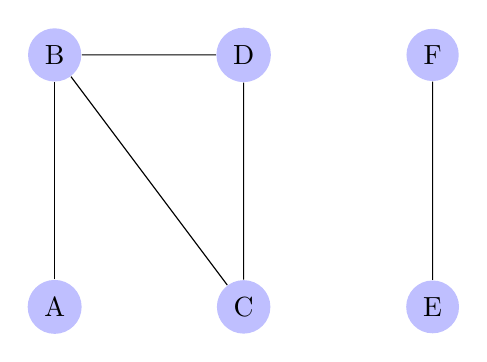
\begin{tikzpicture}
[scale=.8,auto=left,every node/.style={circle,fill=blue!25}]
  \node (n6) at (3,2) {A};
  \node (n4) at (3,6) {B};
  \node (n5) at (6,2) {C};
  \node (n1) at (6,6) {D};
  \node (n2) at (9,2) {E};
  \node (n3) at (9,6) {F};
  \foreach \from/\to in {n6/n4,n4/n5,n5/n1,n2/n3,n4/n1}
    \draw (\from) -- (\to);
\end{tikzpicture}
\caption{En graf, der ikke er et træ.} 
\label{eksempel_notree}
\end{figure}

\noindent Mange anvendelser af træer, kræver at en bestemt knude i en graf fungerer som udgangspunkt. En knude kan indentificeres som en rod, og dermed rodfæste grafen.

\begin{defn}
Et rodfæstet træ er et træ med en knude, der er udnævnt som roden. De resterende knuder er orienteret væk fra roden.
\end{defn}

\noindent Der findes terminologi, der beskriver knudernes forhold til hinanden i en rodfæstet graf. 
Hvis $T$ er et rodfæstet træ, så er en knude $v$, som ikke er roden, $\textit{forælder}$ til en knude $u$, hvis der eksiterer en orienteret kant fra $v$ til $u$ i retningen væk fra roden.
Samtidigt er $u$ $\textit{barn}$ af $v$, og knuder med samme forælder kaldes $\textit{søskende}$. 
$\textit{Forfædrene}$ til $v$ er knuderne på vejen fra roden til $v$, og $\textit{efterkommerne}$ til $v$ er knuderne, der har $v$ som forfader. 
Knuder, der har børn kaldes $\textit{indre knuder}$, og knuder, der ikke har børn kaldes $\textit{blade}$.
Hvis $w$ er en knude i et træ, så er et deltræ med $w$ som rod, træet, det består af $w$ og alle dets efterkommere og alle kanter incidente til efterkommerne.

\begin{exmp}
Betragt træet i Figur \ref{eksempel_rootedtree}. 
For at eksemplificere terminologien, så er roden af træet $a$, og $a$ er forælder til $b$ og $c$, hvilket vil sige, at $b$ og $c$ er børn til $a$, og $b$ og $c$ er hinandens søskende. 
Knuden $b$ er efterkommer af $a$, og den er forfader til $\lbrace d, e, f \rbrace$. 
I grafen er $a$, $b$ og $c$ grafens indre knuder, og mængden af blade er $\lbrace d, e, f, g, h, i \rbrace$. 
Et eksempel på en deltræ af træet i Figur \ref{eksempel_rootedtree} er træet i Figur \ref{eksempel_rootedsubtree}.
Deltræet har $b$ som rod og indeholder efterkommerne af $b$ og kanterne incidente med dem. 
\end{exmp}

\begin{figure}[h]
\centering
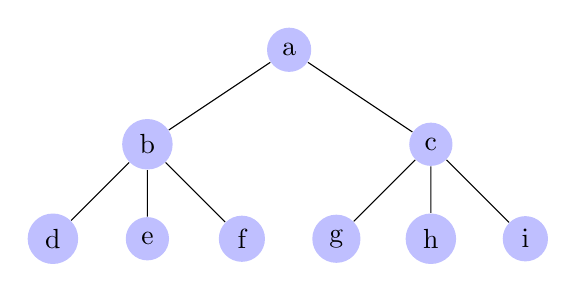
\begin{tikzpicture}
[scale=.8,auto=left,every node/.style={circle,fill=blue!25}]
  \node {a}
  	child{node{b}
  		child{node{d}}
  		child{node{e}}
  		child{node{f}}}
  	child[missing]
  	child[missing]
  	child{node{c}
  		child{node{g}}
  		child{node{h}}
  		child{node{i}}};
\end{tikzpicture}
\caption{Et rodfæstet træ.} 
\label{eksempel_rootedtree}
\end{figure}

\begin{figure}[h]
\centering
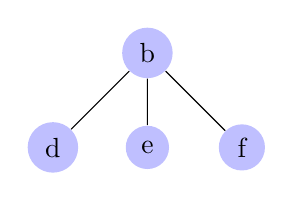
\begin{tikzpicture}
[scale=.8,auto=left,every node/.style={circle,fill=blue!25}]
  \node {b}
  	child{node{d}}
  	child{node{e}}
  	child{node{f}};
\end{tikzpicture}
\caption{Et undertræ med $b$ som rod.} 
\label{eksempel_rootedsubtree}
\end{figure}

\subsection{Udspændende træer}

\begin{figure}[h]
\centering
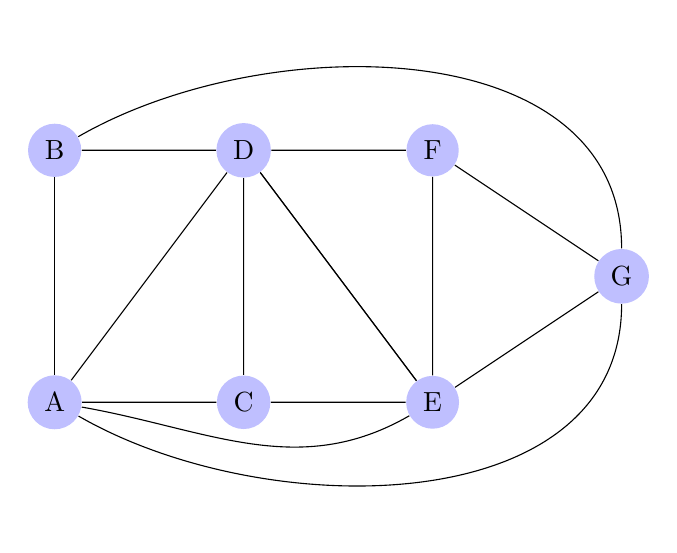
\begin{tikzpicture}
[scale=.8,auto=left,every node/.style={circle,fill=blue!25}]
  \node (n6) at (3,2) {A};
  \node (n4) at (3,6) {B};
  \node (n5) at (6,2) {C};
  \node (n1) at (6,6) {D};
  \node (n2) at (9,2) {E};
  \node (n3) at (9,6) {F};
  \node (n7) at (12,4) {G};
  \foreach \from/\to in {n6/n4,n5/n1,n2/n3,n4/n1,n6/n1,n1/n2,n3/n7,n7/n2,n5/n6,n5/n2,n1/n2,n1/n3}
    \draw (\from) -- (\to);
    \draw (n4) to[out=30,in=90] (n7);
    \draw (n6) to[out=-10,in=-150] (n2);
    \draw (n6) to[out=-30,in=-90] (n7);
\end{tikzpicture}
\caption{123.} 
\label{eksempel_udspaendende}
\end{figure}

%Billede med 4 udspændende træer
\begin{figure}[!htb]
\begin{minipage}{1\linewidth}

\centering
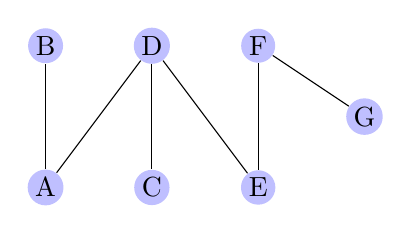
\begin{tikzpicture}
[scale=.45,auto=left,every node/.style={circle,fill=blue!25},inner sep=1pt,minimum size=2pt]
  \node (n6) at (3,2) {A};
  \node (n4) at (3,6) {B};
  \node (n5) at (6,2) {C};
  \node (n1) at (6,6) {D};
  \node (n2) at (9,2) {E};
  \node (n3) at (9,6) {F};
  \node (n7) at (12,4) {G};
  \foreach \from/\to in {n6/n4,n6/n1,n1/n5,n1/n2,n2/n3,n3/n7}
    \draw (\from) -- (\to);
\end{tikzpicture}
\caption{1}
\label{eksempel_udspaendende1}
\end{minipage}

\hfill

\begin{minipage}{1\linewidth}
\centering
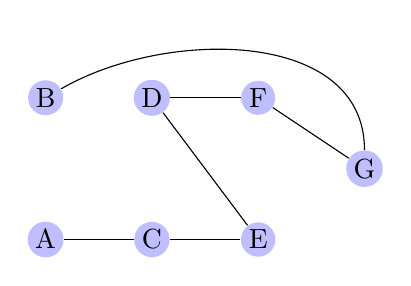
\begin{tikzpicture}
[scale=.45,auto=left,every node/.style={circle,fill=blue!25},inner sep=1pt,minimum size=2pt]
  \node (n6) at (3,2) {A};
  \node (n4) at (3,6) {B};
  \node (n5) at (6,2) {C};
  \node (n1) at (6,6) {D};
  \node (n2) at (9,2) {E};
  \node (n3) at (9,6) {F};
  \node (n7) at (12,4) {G};
  \foreach \from/\to in {n7/n3,n1/n3,n1/n2,n2/n5,n5/n6}
    \draw (\from) -- (\to);
    \draw (n4) to[out=30,in=90] (n7);
\end{tikzpicture}
 \caption{2}
\label{eksempel_udspaendende2}

\end{minipage}

\begin{minipage}{1\linewidth}

\centering
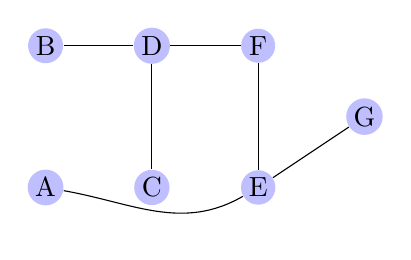
\begin{tikzpicture}
[scale=.45,auto=left,every node/.style={circle,fill=blue!25},inner sep=1pt,minimum size=2pt]
  \node (n6) at (3,2) {A};
  \node (n4) at (3,6) {B};
  \node (n5) at (6,2) {C};
  \node (n1) at (6,6) {D};
  \node (n2) at (9,2) {E};
  \node (n3) at (9,6) {F};
  \node (n7) at (12,4) {G};
  \foreach \from/\to in {n1/n3,n1/n4,n1/n5,n2/n7,n2/n3}
    \draw (\from) -- (\to);
    \draw (n6) to[out=-10,in=-150] (n2);
\end{tikzpicture}
\caption{3}
\label{eksempel_udspaendende3}
\end{minipage}

\hfill

\begin{minipage}{1\linewidth}
\centering
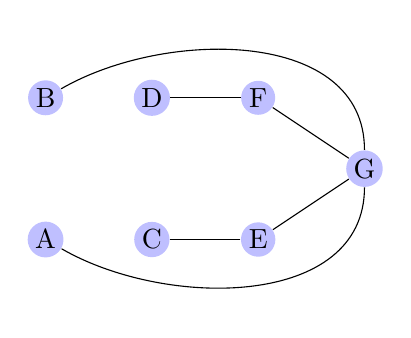
\begin{tikzpicture}
[scale=.45,auto=left,every node/.style={circle,fill=blue!25},inner sep=1pt,minimum size=2pt]
  \node (n6) at (3,2) {A};
  \node (n4) at (3,6) {B};
  \node (n5) at (6,2) {C};
  \node (n1) at (6,6) {D};
  \node (n2) at (9,2) {E};
  \node (n3) at (9,6) {F};
  \node (n7) at (12,4) {G};
  \foreach \from/\to in {n3/n7,n1/n3,n7/n2,n2/n5}
    \draw (\from) -- (\to);
    \draw (n4) to[out=30,in=90] (n7);
    \draw (n6) to[out=-30,in=-90] (n7);
\end{tikzpicture}
 \caption{4}
\label{eksempel_udspaendende4}

\end{minipage}

\end{figure}
\chapter{Traveling Salesperson Problem} \label{chap:TSP}

\section{Introduktion til TSP}

\section{Approksimationsalgoritmer}
TSP er et optimeringsproblem, fordi løsningen består i at finde Hamiltonkredsen med mindst mulig vægt i en graf. 
Af samme grund er problemet også et minimeringsproblem. 
I et minimeringsproblem ønskes der at finde en løsning $S$, hvor $d(S)$ er mindst mulig.
Nogle gange skal der gøres brug af en ikke-polynomiel algoritme for at finde den minimale løsning.
Da kan der gøres brug af approksimationsalgoritmer.

\begin{defn}\label{def:apk}
Lad $S$ være den optimale løsning til et minimeringsproblem. En $k$-approksimationsalgoritme er en polynomiel algoritme, der returnerer en mulig løsning $S'$, således
\begin{align*}
d(S') \leq k \cdot d(S),
\end{align*}
hvor $k$ er approksimationskonstanten, og $k \in \mathbb{R}_{\geq 1}$.
\end{defn}

Tilsvarende findes der approksimationsalgoritmer til at løse maksimeringsproblemer med $0 < k \leq 1$. \citep{approksalg}

\section{TSP}
\section{Løsningsalgoritmer}

Der findes indtil flere løsningsalgoritmer til at løse TSP. Det viser sig dog imidlertid, at der ikke er nogen let måde, at løse problemet på. Som tidligere nævnt, er det nødvendigt at ty til approksimationsalgoritmer for at have en chance for at finde en nogenlunde brugbar løsning.

Den mest umiddelbart løsningsalgoritme til at finde en korteste Hamiltonkreds rundt i en graf, finder samtlige mulige Hamiltonkredse i grafen. Til hver af disse kredse beregnes den samlede vægt, og til sidst sammenlignes alle disse samlede vægte, for at finde den Hamiltonkreds, som har den mindste samlede vægt. Denne algoritme er i pseudokode beskrevet i Algoritme \ref{brute_force}.

\begin{algorithm}
\caption{Brute-force algoritmen}
\label{brute_force}
\textbf{procedure} Find korteste Hamiltonkreds i grafen $G$ med $\alpha$ Hamiltonkredse.

Bestem alle Hamiltonkredse, $H_k$, i $G$, og lad $H_{ki}$ betegne den $i$'te Hamiltonkreds. \\
\textbf{for} $i:=1$ til $\alpha$ \\
$\-$ $\-$ $\-$ $\-$ $\-$ $\-$
Bestem $d(H_{ki})$ \\
$min := H_{k1}$ \\
\textbf{for} $i:=2$ til $\alpha$ \\
$\-$ $\-$ $\-$ $\-$ $\-$ $\-$
\textbf{hvis} $min > H_{ki}$ \textbf{så} $min := H_{ki}$ \\
\textbf{returnér} $min$ $\lbrace$ $min$ er den korteste Hamiltonkreds i $G$ $\rbrace$
\end{algorithm}

Denne algoritme vil altid finde den korteste Hamiltonkreds i en komplet graf $G$, men kræver meget processorkraft at gennemføre, selv for grafer med relativt få knuder \citep{dmat}.

\begin{thm}
Den værst mulige tidskompleksitet af Brute-force Algoritmen er $O(n!)$.
\end{thm}

\begin{proof}
Lad $G$ være en komplet graf med $n$ knuder og $n \geq 3$. I denne graf er der så $(n-1)!$ forskellige Hamiltonkredse, idet de $n-1$ punkter kan arrangeres på $(n-1)!$ forskellige måder. Derfor har algoritmen allerede her en værst mulig tidskompleksitet på $O(n!)$ idet $(n-1)!$ er $O(n!)$. 

Herfter foretager algoritmen en lineær søgning, som jf. Eksempel \ref{eks_lin_soeg} har en værst mulig tidskompleksitet på $\Theta(n)$, og spiller derfor ingen rolle i algoritmens samlede kompleksitet.
\end{proof}

Brute-force algoritmen har således en kompleksitet, der er voldsom stor selv ved relativt få knuder i $G$.

\begin{exmp}
I den komplet graf, $G$, med $20$ knuder, har brute-force algoritmen en værst mulig tidskompleksitet på $$20! = 2432902008176640000,$$ hvorfor algoritmen tydeligvis allerede ved $20$ knuder er håbløs.
\end{exmp}

Derfor er approksimationsalgoritmer nødvendige, for at løse problemet. Som tidligere beskrevet, vil disse algoritmer \textit{ikke} finde den optimale løsning, men en løsning, som ligger indenfor en vis konstant grænse. I denne rapport vil Dobbelttræ-algoritmen anvendes til at løse TSP. 

\subsection{Dobbelttræ-algoritmen}
Dobbelttræ-algoritmen forudsætter, at grafen, som Hamiltonkredsen skal findes i, er komplet metrisk. For sådanne grafer kan der imidlertid foretages en \textit{genvej}, som defineres i Definition \ref{def_genvej}.

\begin{defn}
Lad $G$ være en komplet, metrisk graf med $n$ knuder og $n \geq 3$. I $G$ findes en vej, $P = v_0, v_1,...,v_{i-1}, v_i, v_{i+1},...,x_{n-1},x_n$ hvor $1 \leq i \leq n-1$. \\
I $P$ findes så to kanter $e_i = \lbrace x_{i-1}, x_i \rbrace$ og $e_{i+1} = \lbrace x_i, x_i+1 \rbrace$, så $e_i \cap e_{i+1} = x_i$.
Der findes så en trekant $\Delta_i = \lbrace e_i, e_{i+1}, e_s \rbrace$ i $G$, hvor $e_s = \lbrace x_{i-1}, x_{i+1} \rbrace$.
Da kan der dannes en genvej i $P$ via $e_s$ således en ny vej, $P'=v_0, v_1,...,x_{i-1},x_{i+1},...,x_{n+1},x_n$, dannes.
Idet $G$ er metrisk opfylder den trekantsuligheden, så $d(e_s) \leq d(e_i) + d(e_{i+1})$ og dermed er $d(P') \leq d(P)$.
\label{def_genvej}
\end{defn}

Dobbelttræ-algoritmen begynder med, i en komplet, metrisk graf $G$, at finde et minimalt udspændende træ, $T$, som kan findes ved hjælp af Prims Algoritme. Når $T$ er fundet, fordobles alle kanter i $T$, som så danner en multigraf $D$. Graden af alle knuder i denne grad må være lige, hvorfor der må eksistere en Eulerkreds i $D$, jf. Sætning \ref{Eulerkreds_multigraf}. Eulerkredsen dannes ved Algoritme \ref{algoritme_euler}.  I denne Eulerkreds skydes der genvej, for at opnå en Hamiltonkreds, $H$. Denne algoritme er sammenfattet i Algoritme \ref{dt_algo}. 

\begin{algorithm}[h]
\caption{Dobbelttræ-algoritme}
\label{dt_algo}
\textbf{procedure} En metrisk komplet graf, $G$ \\
Find minimalt udspændende træ, $T$, i $G$ $\lbrace$ Prims Algoritme $\rbrace$. \\
$D := T$ \\
\textbf{for} kant \textbf{i} $D$ \\
$\-$ $\-$ $\-$ $\-$ $\-$ $\-$
dublér kant \\
Find Eulerkreds, $E$, i $D$ \\
Skyd genvej i $E$ for at opnå Hamiltonkredsen, $H$ \\
\textbf{returnér} $H$ $\lbrace$ $H$ er Hamiltonkreds i $G$ $\rbrace$
\end{algorithm}

Dobbelttræ-algoritmen approksimerer den Hamiltonkreds, som er af lavest mulig vægt.

\begin{thm}
Dobbelttræ-algoritmen er en 2-approksimationsalgoritme.
\end{thm}

\begin{proof}
Lad $H'$ være Hamiltonkredsen af lavest muligt vægt i grafen $G$ og $H$ være den Hamiltonkreds, som Dobbelttræ-algoritmen finder ved genvej i Eulerkredsen $E$. Da må der gælde, at $$d(H)\leq d(E).$$ 
Idet Eulerkredsen, $E$, er dannet ved at dublere alle kanter i det minimalt udspændende træ, $T$, må der gælde, at $$d(E) = 2d(T).$$
Idet enhver Hamiltonkreds ved fjernelse af en kant danner et udspændende træ, må der i $H'$'s tilfælde gælde, at $d(T) \leq d(H')$. Heraf følger det, at $$2d(T) \leq 2d(H').$$
Derfor må der gælde, at $$d(H) \leq 2d(H'),$$ hvorfor Dobbelttræ-algoritmens fundne Hamiltonkreds, $H$, ikke har en vægt større end $2d(H')$. 
\end{proof}

\subsection{Kompleksitet af Dobbelttræ-algoritmen}
Dobbelttræ-aalgoritmen er en approksimationsalgoritme, som det er bevist ovenfor. Derfor må det formodes, at den har en lavere kompleksitet end Brute-force Algoritmen havde.

\begin{thm}
Dobbelttræ-algoritmen har en værst mulig tidskomplesitet på $O(n^3)$.
\end{thm}

\begin{proof}
Dobbelttræ-algoritmen gennemkører først Prims Algoritme, som er $O(n^3)$, jf. Sætning \ref{prim_kompl}. 
Derefter fordobler algoritmen samtlige sider i træet, som Prims Algoritme har dannet. Denne tilfører kompleksiteten $O(n)$.
Så gennemkører Dobbelttræ-algoritmen algoritmen for dannelsen af en Eulerkreds, som har lineær værst mulig tidskompleksitet, altså også $O(n)$.
Slutteligt vil Dobbelttræ-algoritmen skyde genvej ved at gennemgå den dannede Hamiltonkreds, hvilket også har lineær værst mulig tidskompleksitet. 
Derfor må den værst mulige tidskompleksitet af Dobbelttræ-algoritmen være $O(n^3)$.
\end{proof}

Dobbelttræ-algoritmen viser sig altså at være af polynomiel værst mulig tidskompleksitet, hvorfor denne noget hurtigere vil finde en kort Hamiltonkreds i grafen. Dog er det på kompromis at, at det ikke nødvendigvis er den korteste Hamiltonkreds i $G$.

\begin{exmp}
I den komplette graf, $G$, med $20$ knuder, har Dobbelttræ-algoritmen en værst mulig tidskompleksitet på $$20^3 = 8000,$$ og er derfor markant hurtigere end Brute-force Algoritmen.
\end{exmp}






\chapter{Diskussion}

Tidskompleksiteten angivet ved Store-$\Theta$ notation estimerer tiden, det tager en algoritme at løse et problem, i takt med at inputtet stiger. 
Den faktiske computertid varierer, og nutidens hurtigste computere kan udføre en operation i en algoritme på $10^{-11}$ sekunder. \cite{dmat}.
En Brute Force algoritme til at løse Travelling Salesperson Problem har faktoriel tidskompleksitet, $\Theta(n!)$, hvor der estimeres en anvendelse af maksimalt $n!$ operationer.
Med nutidens hurtigste computere, vil det tage algortime urealistisk lang tid løse problemet, hvis inputtet når over eksempelvis $n=20$, hvilket ses i Tabel \ref{tab_algtsp}. Det ses samtidigt, at Dobbelttræ algoritmen har en væsentlig lavere gennemløbstid, og selv i større grafer vil algoritmen køres på under et millisekund. 

\begin{table}[h]
 \centering
  \begin{tabular}{|c|c|c|c|c|}
   \hline
   Algoritme & Kompleksitet & $n=10$ & $n=20$ & $n=30$\\
   \hline
   Brute Force & $\Theta(n!)$ & $3,6 \cdot 10^{-11}$ sek & $281,6$ dage & $8,4 \cdot 10^{13}$ år \\
   \hline
   Dobbelttræ & $\Theta(n^3)$ & $1,0 \cdot 10^{-9}$ sek & $8,0 \cdot 10^{-8}$ sek & $2,7 \cdot 10^{-7}$ sek \\
   \hline
  \end{tabular}
 \caption{Gennemløbstiden afhængig af inputstørrelsen for løsningsalgortimerne, hvor det er antaget, at der udføres én operation per $10^{-11}$ sekunder.} \label{tab_algtsp}
\end{table}

Grundet den urealistisk lange gennemløbstid vil det være urentabelt at bruge ressourcer på at implementere en Brute Force algortime for at løse Travelling Salesperson Problem i en større graf, selvom Brute Force algortimen med sikkerhed kan finde Hamilton kredsen med mindst vægt. 
I stedet kan der indgås et kompromis med algoritmens præcision. 

Ved at anvende Dobbelttræ algoritmen findes der en approksimation på løsningen i stedet for den optimale løsning, men tilgengælg forbedres gennemløbstiden markant, som det ses Tabel \ref{tab_algtsp}. 
Den forbedrede hastighed for at køre algoritmen gør det muligt at approksimere løsninger af Travelling Salesperson Problem, selv når mange byer skal besøges. 
Medfører approksimationen ikke en uacceptabel stor fejl, kan det være en  fordel at løse problemet ved at gå på kompromis med algoritmens præcision.

Udover egenskaberne at være hurtig at udføre og præcis set i forhold til at finde den optimale løsning kan det overvejes, hvorvidt en algoritme skal kunne løse et givent problem i alle tilfælde. 
Der laves et kompromis, da Travelling Salesperson Problem afgrænses til det metriske tilfælde, for at der kan findes en løsningsalgoritme. For at løse andre typer af Travelling Salesperson Problem, anvendes andre løsningsalgoritmer. 
\chapter{Perspektivering}
TSP-problemet består af flere undergrupper af algoritmiske problemer, som afhænger af hvilke type svar der ledes efter. Søger man efter flere korrekte svar, kaldes problemet for et søgningsproblem. Leder man efter en optimal løsning, kaldes problemet for et optimeringsproblem. Et eksempel på dette, kan være at man leder efter den kortest mulige vej, hvilket er den version af TSP der er blevet arbejdet med i dette projekt. Optimeringsproblemer og søgeproblemer kaldes også for evalueringsproblemer eftersom evalueringsproblemer altid har enestående løsninger .

En anden type problemer er beslutningsproblmer, hvor der blot søges ét af to svarmuligheder, ja eller nej. Denne version af TSP tager endnu et input, netop en samlet vægt, og der skal så tjekkes for om der eksisterer en hamiltonkreds i grafen med mindre samlet vægt end denne.

Forskellige versioner af TSP kan muligvis have forskellige løsningsalgoritmer. Specielt ligger beslutningsversionen af TSP ikke i kompleksitetsklassen $NP-hard$ som optimeringsversionen gør, men i klassen $NP-complete$.


En anden mulig perspektivering til TSP kan være CPP (Chinese postman problem), som blev fremsat i 1960'erne, af den daværende 26 årige kinesiske matematikker Mei-Ko Kwan. Problemet går ud på, at en postbud skal levere post og ønsker, at skulle gå mindst muligt, altså den korteste distance. Postbuddet skal gå langs alle veje i området da der formenligt skal afleveres post til alle husstande. Buddet starter og slutte ved posthuset,  altså i samme punkt. Modsat salgspersonen i TSP,så skal postbuddet  forbi alle veje i et vejnet for at kunne levere post, mens salgspersonen, i TSP, kun skal finde den korteste vej fra by til by, og altså ikke skal forbi alle veje. 
Vejnetværket som postbuddet skal benytte sig af, kan omdannes til en graf. Mere præcist en vægtet graf, hvor vægtene for eksempel kan repræsenterer længden af hver vej. 
Det er nemt at udregne længden af postmandens rute, hvis der er lige antal kanter i alle af grafens punkter, eftersom at man dermed kan skabe en Eulerkreds. Eulerkredsen betyder at man kun skal krydse samme kant præcis en gang, og dermed er det lige meget hvilken vej man vælger.   
Indholder grafen et lige antal ulige kanter, så betyder det at der ikke længere kan være en eulerkreds, og dermed skal buddet gennem flere kanter mere end en gang. For at udregne/finde ud af hvad den korteste vej skal være, kan man gøre brug af Chinese postman algoritmen, som kan løses på polynomisk tid.

% Appendicer indsættes inde i en appendices-blok og bliver nummereret med
% bogstaver i stedet for tal
\begin{appendices}
  % \include{incl/app/appendix1}
  % \include{incl/app/appendix2}
  % ..
\end{appendices}

% Dokumentets 'back matter' er til ekstra ting som f.eks. litteraturlisten.
% Overskrifter bliver ikke nummereret her.
\backmatter

% Automatisk litteraturliste baseret på, hvilke kilder, der er blevet refereret
% til i løbet af rapporten.
\bibliographystyle{plainnat}
\bibliography{
  incl/bib/books,
  incl/bib/articles,
  incl/bib/software
}

\end{document}
